\documentclass[a4paper, 12pt]{report}
    \parindent=1em
    \parskip=1pt
    \usepackage[font=footnotesize, labelfont=bf]{caption}  % bold caption
    %\usepackage[usenames,dvipsnames]{color}  % not compatible with knitr yet..
    \usepackage{xcolor}  % highlighting.
    \usepackage{enumerate}
    \usepackage[round]{natbib}
    \usepackage{graphicx}  % rotate text
    \usepackage{listings}  % fancyvrb doesn't have word wrap..
        \lstset{
            basicstyle=\small\ttfamily,
            columns=flexible,
            breaklines=true,
            captionpos=t,  % sets the caption-position to bottom
            numbers=left,  % line numbers on the left
            frame=single,  % adds a frame around the code
            fontadjust=true,
            escapechar=|
            %language=HTML,
            aboveskip=0pt,
            belowskip=5pt,
        }
    \usepackage{url}
	\usepackage[htt]{hyphenat}  % enable hyphenation of TT text
    \usepackage{tikz}
      \usetikzlibrary{decorations.text, arrows}  % decoration for for curved text
      \usetikzlibrary{positioning}  % for positioning nodes
    \usepackage{hyperref}
    \usetikzlibrary{shapes.geometric, arrows}
    \usepackage[export]{adjustbox}  % better image alignment & scale
    \usepackage{titlesec}  % chapter
        \titleformat
        {\chapter} % command
        [display] % shape
        {\bfseries\Large\itshape} % format
        {} % label
        {-15ex} % sep
        {
            \rule{\textwidth}{1pt}
            \vspace{1ex}
            \centering
        } % before-code
        [
        \vspace{-2ex}%
        \rule{\textwidth}{0.3pt}
        ] % after-code

%%%%% flow chart configuration %%%%%
\tikzstyle{simple} = [rectangle, rounded corners, text width=3cm, text centered, font=\small, draw=black, align=center, fill=green!20]
\tikzstyle{startstop} = [rectangle, rounded corners, minimum width=3cm, minimum height=1cm, text centered, draw=black, fill=green!20, font=\small]
\tikzstyle{process} = [rectangle, minimum width=2cm, minimum height=1cm, text centered, text width=1cm, draw=black, font=\small]
\tikzstyle{decision} = [diamond, minimum width=2cm, minimum height=1cm, text centered, draw=black, fill=green!30, font=\small]
\tikzstyle{arrow} = [thick,->,>=stealth]
\tikzstyle{line} = [thick,-,>=stealth]

\title{\textbf{Invertible Reproducible Documents}}
\author{Eric Lim}
\date{\today}

%\renewcommand\thesection{\arabic{section}}  % remove chapter numbering in section

\begin{document}
  \maketitle


%------------------------------------------------------------------------------
%------------------------------------------------------------------------------
%---------------------------- Chapter: Motivation -----------------------------
%------------------------------------------------------------------------------
%------------------------------------------------------------------------------
\chapter{Motivation}
\label{ch:motiv}

%<<setup, echo=FALSE>>=
%opts_chunk$set(comment = NA, prompt = TRUE, tidy = FALSE, background='white')
%options(prompt = "R> ")
%knit_theme$set("print")
%@

\textbf{Knitr} \citep{knitr} is a wonderful package that enables dynamic report generation with R. It allows integration of R code into LaTeX, LyX, HTML, Markdown, AsciiDoc, and reStructuredText documents through the concepts of literate programming \citep{knu84}, which involves interaction between code and documentation for report generation. The main purpose of \textbf{knitr} follows an important idea in academic research that the ideal research paper or report must encompass the entire computational environment used to produce the results in the paper such as the code so that the same results can be reproduced using the same computational environment. The importance of reproducibility can be further extended to be applied in the entire area of academia \citep{lee01}.

\begin{figure}[h]
\centering
  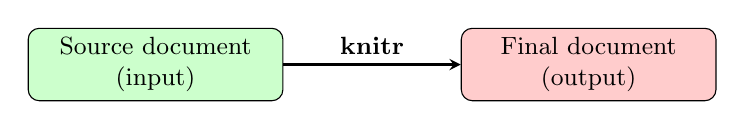
\begin{tikzpicture}[node distance=3cm]
    \node(in)[simple]{Source document \\ (input)};
    \node(out)[simple, fill=red!20, right of=in, xshift=2.5cm]{Final document \\ (output)};
    \draw[arrow](in)--node[anchor=south]{\small{\textbf{knitr}}} (out);
  \end{tikzpicture}
  \caption{Unidirectional document generation by \textbf{knitr}}
  \label{fig:1}
\end{figure}

While there are tremendously important ideas to consider and many advantages, the process of generating R code embedded documents using \textbf{knitr} is almost always a one-way trip (Figure \ref{fig:1}), meaning source documents (as input) can only generate final documents (as output), not the other way around. This is simply due to the fact that \textbf{knitr} is designed with intention to dynamically generate reports, not to extract displayed R code in final documents in order to generate source documents.

Consider a situation where a \emph{consultant} provides reports as reproducible documents and a \emph{client} is to read or review the reports. In this situation, it is often difficult for the consultant to receive feedback from the client efficiently. Since it is impossible to convert back from final documents to source documents, the client would have to provide his or her feedback by either writing physically on the printed copy of the final report or by electronic means such as through exchanging e-mails. The document provider, then, has to rectify the source documents accordingly, only to repeat the process of generating and presenting the report to the client. This process often has to be repeated until final correction can be achieved. As we can see, it can quickly become tedious.

We believe this is relevant to the field of statistics as similar situations mentioned above can often arise. Interaction between clients and consultants is crucial for statisticians and any possible factor to deteriorate the relationship with clients is best avoided. Therefore, we want to avoid this issue by a more efficient document generation workflow.

A possible solution is to allow clients to interact directly with the final documents and edit them. Then consultants can merge the changes and make final adjustments to generate new reports efficiently. In order to achieve this, reports must be \emph{invertible}, as well as reproducible, that is, final reports must be able to be converted into the source document format without introducing any change from the inversion process itself.

\begin{figure}[h]
\centering
  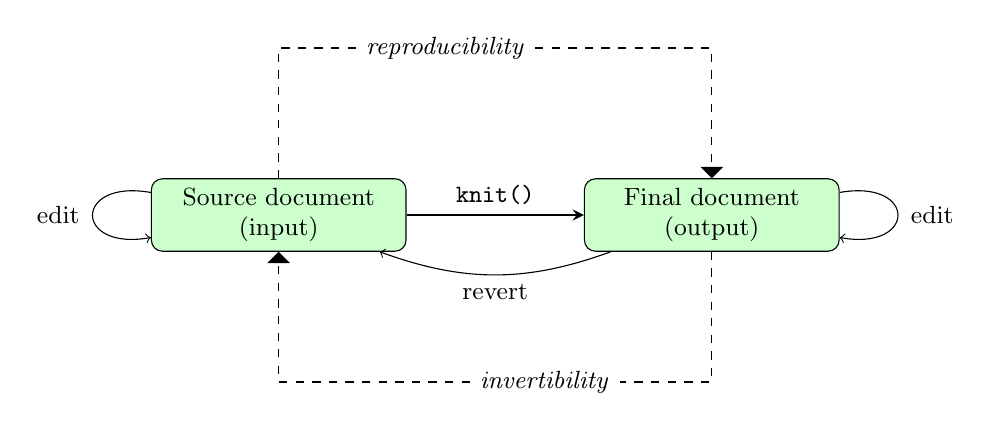
\begin{tikzpicture}[node distance=3cm]
    \node(in)[simple]{Source document \\ (input)};
    \node(out)[simple, right of=in, xshift=2.5cm] {Final document \\ (output)};
    \draw [arrow] (in)--node[anchor=south]{\small{\texttt{knit()}}} (out);
    \draw [->] (out) to [bend left=20] node[anchor=north] {\small{revert}} (in);
    \draw [->] (in) to [loop left, in=190, out=170, distance=1cm] (in) node[anchor=north, left of=in, xshift=2mm] {\small{edit}};
    \draw [->] (out) to [loop right, in=350, out=10, distance=1cm] (out) node[anchor=west, right of=out, xshift=-2mm] {\small{edit}};
    %
    \node(re) [above right of=in] {\small{\emph{reproducibility}}};
    \node(inv) [below left of=out] {\small{\emph{invertibility}}};
    \draw [dashed] (in)|-(re);
    \draw [dashed, arrows={-triangle 90}] (re)-|(out);
    \draw [dashed] (out)|-(inv);
    \draw [dashed, arrows={-triangle 90}] (inv)-|(in);
    %
    %\def\myshift#1{\raisebox{1ex}}  % so the text doesn't touch the line of arrow
    %\draw [dashed, ->, postaction={decorate, decoration={text along path, text align=center, text={|\small\myshift|reproducibility}}}] (in) to [bend left=60]  (out);
    %\def\myshift#1{\raisebox{-2.5ex}}
    %\draw [dashed, ->, postaction={decorate, decoration={text along path, text align=center, text={|\small\myshift|invertibility}}}] (out) to [bend left=60] (in);
    
    %\draw [dashed, ->] (in) to [bend left=60] node[anchor=north] {reproducibility} (out);
    %\draw [dashed, ->] (out) to [bend left=60] node[anchor=south] {invertibility} (in);
  \end{tikzpicture}
  \caption{Invertible reproducible workflow}
  \label{fig:2}
\end{figure}

This report introduces a possible workflow that can be utilised effectively in the aforementioned situation. The main focus of the project is in achieving this hypothetical round trip and exploring possible issues associated with it. Generalising the workflow by improving the robustness and efficiency of the functions involved has only been considered to a level that has been manageble under the time given for the project. Hence, it has been possible to devise two separate strategies to deal \emph{specifically} with two different document types under the allowed time. The phase 1 of this report will discuss primarily on dealing with HTML-based documents and the second phase will focus on Markdown-based documents.



%------------------------------------------------------------------------------
%------------------------------------------------------------------------------
%------------------------------ Chapter: R HTML -------------------------------
%------------------------------------------------------------------------------
%------------------------------------------------------------------------------
\chapter{Phase 1: R HyperText Markup Language}
\begin{figure}[h]
\centering
  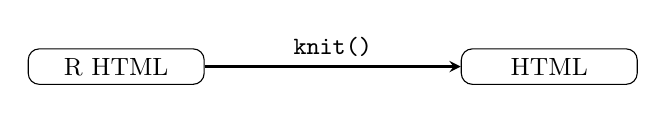
\begin{tikzpicture}[node distance=3cm]
    \node(in)[simple, fill=white, text width=2cm]{R HTML};
    \node(out)[simple, fill=white, text width=2cm, right of=in, xshift=2.5cm]{HTML};
    \draw[arrow](in)--node[anchor=south]{\small{\texttt{knit()}}} (out);
  \end{tikzpicture}
\end{figure}

\section*{Introduction}
\label{sec:3.1}
The primary objective of the initial phase is to design and achieve a complete reproducible, invertible workflow. There are many obstacles that limit the possibility of devising an invertible workflow. A sizable one of these problems is that converting (or inverting) between two different document formats requires a tremendous amount of a particular resource that we were limited on; \emph{time}.

Out of the many formats that \textbf{knitr} supports, R HTML is the format we have chosen for the objective. There are two main reasons for this choice; R HTML does not require conversion between two document formats and it allows the use of powerful text processing tools, all of which increase our chance of accomplishing a reproducible, invertible workflow.

%-------------------------------------------------------------------------------
\subsubsection*{Support of unified format}
In \textbf{knitr}, R HTML-based documents are \emph{knitted} to produce HTML-based documents. The \emph{only} difference between these two document formats is that R HTML-based documents contain sections of lines of R code, known as R Code Chunks. Here is an example of a simple R Code Chunk:
\begin{lstlisting}[numbers=none, frame=none]
<!--begin.rcode
plot(cars)
end.rcode-->
\end{lstlisting}
By using the function, \texttt{knit()}, in \textbf{knitr}, the R Code Chunk is run in R to produce output (a plot for the previous example). The R code, \texttt{plot(cars)}, and the output plot are, then, enclosed separately in nested \texttt{div} elements in the final HTML-based document.

\textbf{Knitr} generates HTML documents, as output, from \emph{HTML-based} R HTML documents, as input. In other words, the document generation process does not involve conversion between two distinct document formats. The source document format is essentially the same as the final document format.

By this property, difficulties associated with inverting a document format back into a different format can be minimised and the chance of inverting is increased.

%-------------------------------------------------------------------------------
\subsubsection*{Availability of tool sets}
HTML is markup language very similar to XML. This means powerful XML-based tool sets, such as XPath \citep{xpath}, are available for use to manipulate the HTML documents effectively. The R package, \textbf{XML} \citep{xml}, is used to provide these XML-based tool sets in R.

%-------------------------------------------------------------------------------
\subsubsection*{Demonstration}
Here is a brief demonstration of how an R HTML document can be used to generate a HTML document.

Listing \ref{lst:2.1} is the code structure of the source document, \texttt{example1.Rhtml}. The highlighted text (lines 8--10) is an R Code Chunk. The option, \texttt{echo=FALSE}, is used to hide the R code in the final document.
\definecolor{c}{HTML}{CCFF00}
\newcommand{\hl}[3][black]{{\fboxsep0.5pt\colorbox{#2}{\color{#1} #3}}}
\begin{lstlisting}[caption={\texttt{example1.Rhtml}}, escapechar=\|, label={lst:2.1}]
<!DOCTYPE html>
<html>
<head>
</head>
  <body>
    <h1>Example</h1>
    <p>Summary of the cars data:</p>
    |\hl{c}{<!--begin.rcode echo=FALSE}|
    |\hl{c}{summary(cars)}|
    |\hl{c}{end.rcode-->}|
  </body>
</html>
\end{lstlisting}

The following R code is used to \emph{knit} the source document, \texttt{example1.Rhtml}, to generate the final document, \texttt{example1.html}:
\begin{lstlisting}[numbers=none, frame=none]
> library(knitr)
> knit("example1.Rhtml")
\end{lstlisting}

Listing \ref{lst:2.2} shows the code structure of the final document, \texttt{example1.html}. The R code from line 9 of Listing \ref{lst:2.1} is run in R to produce the result seen in lines 13--19 of Listing \ref{lst:2.2}. Cautions must be taken as the code in Listing \ref{lst:2.2} has been tidied up with line endings to enhance readability. The actual untidied code consists of long lines that usually require text-wrap to fit into the page.
\begin{lstlisting}[caption={(tidied) \texttt{example1.html}}, escapechar=\|, label={lst:2.2}]
<!DOCTYPE html>
<html>
<head>
  <style type="text/css"> ... </style>
</head>
  <body>
    <h1>Example</h1>
    <p>Summary of the cars data:</p>
    <div class="chunk" id="unnamed-chunk-1">
      <div class="rcode">
      <div class="output">
        <pre class="knitr r">
          ##      speed           dist    
          ##  Min.   : 4.0   Min.   :  2  
          ##  1st Qu.:12.0   1st Qu.: 26  
          ##  Median :15.0   Median : 36  
          ##  Mean   :15.4   Mean   : 43  
          ##  3rd Qu.:19.0   3rd Qu.: 56  
          ##  Max.   :25.0   Max.   :120
        </pre></div>
      </div></div>
  </body>
</html>
\end{lstlisting}

Figure \ref{fig:2.1} shows what \texttt{example1.html} will look like in a web browser.
\begin{figure}[h!]
% wkhtmltopdf
\fbox{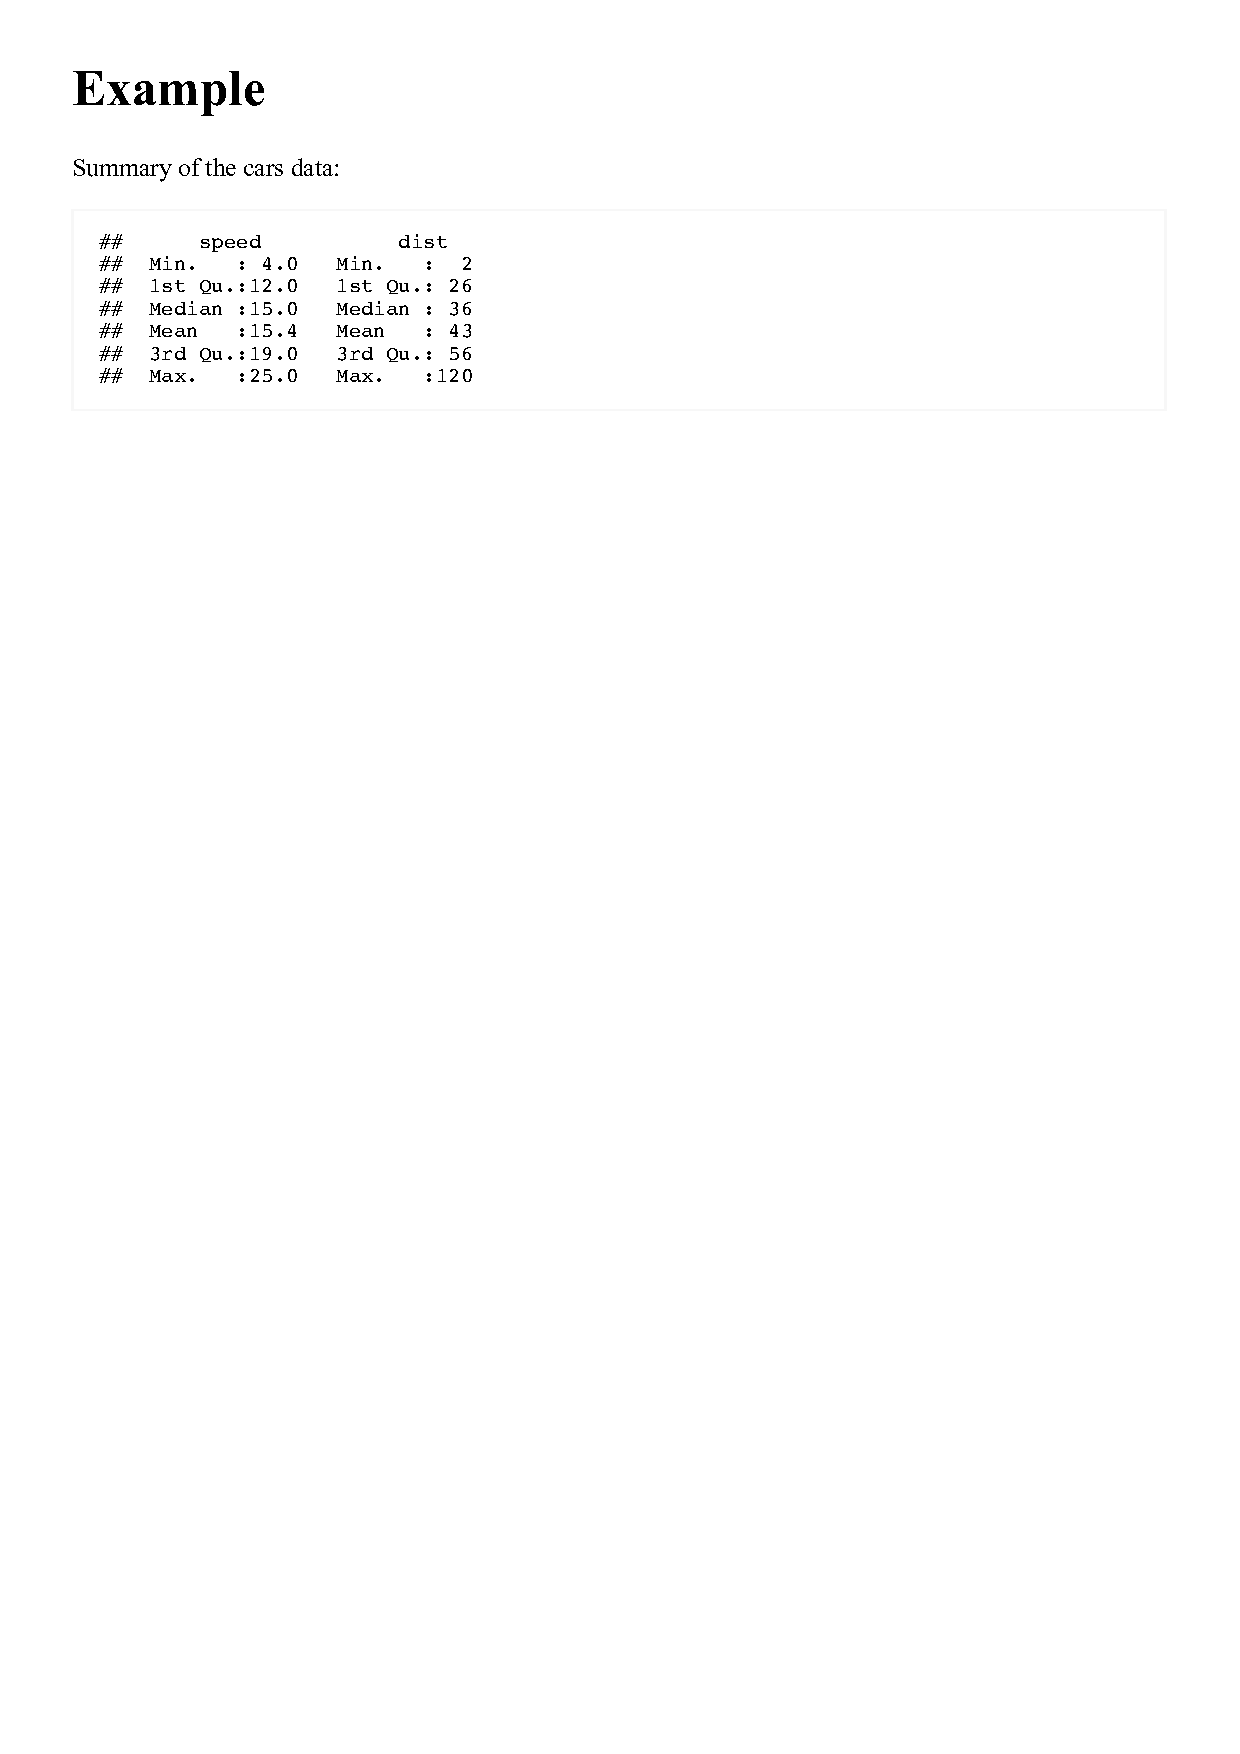
\includegraphics[trim=0cm 22.5cm 0cm 1cm,clip=true,width=1.1\textwidth,center]{example1}}
\caption{\texttt{example1.html} in a browser}
\label{fig:2.1}
\end{figure}

%------------------------------------------------------------------------------
%--------------------------------- Overview -----------------------------------
%------------------------------------------------------------------------------
\pagebreak
\section*{Overview}
\label{sec:overview}

A complete cycle of the invertible workflow consists of six stages. Each stage is involved primarily with text processing, along with an occasional use of XPath.

The actual code for the functions can be found in \url{https://github.com/elim1988/honours-project}.
% Organise my github...

\begin{figure}[h!]
\centering
  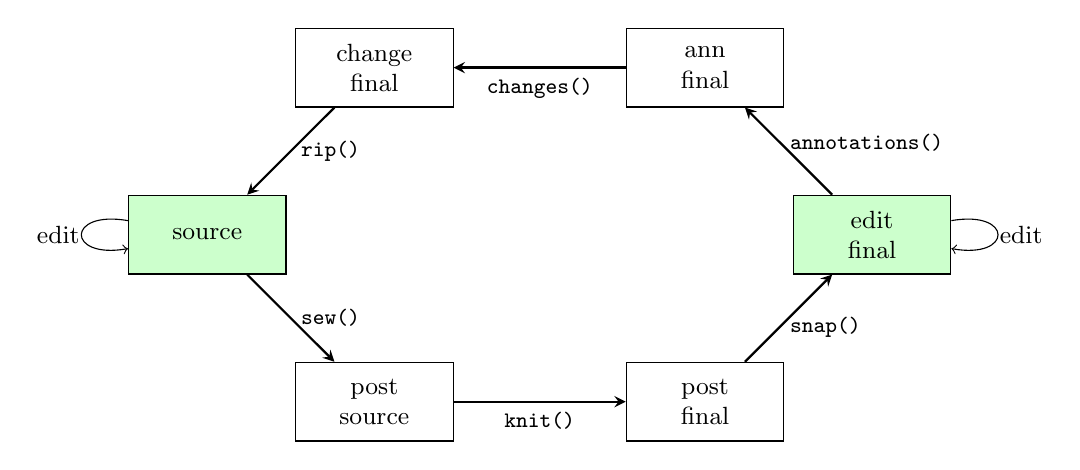
\begin{tikzpicture}
    \node(start)[process, fill=green!20] {source};
    \node(sew)[node distance=3cm, process, below right of=start] {post source};
    \node(knit)[node distance=4.2cm, process, right of=sew] {post final};
    \node(snap)[fill=green!20, node distance=3cm, process, above right of=knit] {edit final};
    %\node(browser)[simple, right of=snap, xshift=2cm]{browser:\\upload, edit, save};
    \node(anno)[node distance=3cm, process, above left of=snap] {ann final};
    \node(chgs)[node distance=4.2cm, process, left of=anno] {change final};
    \draw[arrow](start)--node[anchor=west] {\footnotesize{\texttt{sew()}}} (sew);
    \draw[arrow](sew)--node[anchor=north] {\footnotesize{\texttt{knit()}}} (knit);
    \draw[arrow](knit)--node[anchor=west, pos=0.4] {\footnotesize{\texttt{snap()}}} (snap);
    \draw[arrow](snap)--node[anchor=west, pos=0.6] {\footnotesize{\texttt{annotations()}}} (anno);
    \draw[arrow](anno)--node[anchor=north]{\footnotesize{\texttt{changes()}}} (chgs);
    \draw[arrow](chgs)--node[anchor=west] {\footnotesize{\texttt{rip()}}} (start);
    \draw [->] (start) to [loop left, in=190, out=170, distance=8mm] node[anchor=east, xshift=1mm] {\small{edit}} (start);
    \draw [->] (snap) to [loop right, in=350, out=10, distance=8mm] node[anchor=west, xshift=-1mm] {\small{edit}} (snap);
    %\draw[arrow] (snap) to [out = 30, in = 120, looseness = 1] (browser);
    %\draw[arrow] (snap) to [bend left = 30] (browser);
    %\draw[arrow] (browser) to [bend left = 30] (snap);
    %
    %\draw[line, dashed](rip)-|(repeat);
    %\draw[arrow, dashed](repeat)|-(start);
  \end{tikzpicture}
\caption{The reproducible, invertible workflow}
\label{fig:4}
\end{figure}

%-------------------------------------------------------------------------------
\subsubsection*{Loss of information}
Processing of a source document into a final document can be associated with loss of information from the source document. For example, the original R code in line 9 of Listing \ref{lst:2.1} does not appear in the final document (Listing \ref{lst:2.2}). As a solution, a source document undergoes a pre-processing step where each R Code Chunk is copied in such a way that the original R Code Chunks are perfectly preserved throughout the stages of the workflow and are retainable after a complete cycle.

The pre-processing task is carried out by the function, \texttt{sew()}.

%-------------------------------------------------------------------------------
\subsubsection*{Gain of information}
As opposed to losing information, the document generation process can result in gain of new information. For example, lines 9--19 of Listing \ref{lst:2.2}, which correspond to the output generated from the original R code in line 9 of Listing \ref{lst:2.1}, only exist in the post-processed (final) document. The sections of newly gained information, i.e., the output of R Code Chunks, may seem editable to the client.

However translating changes made on the gained information in the final document to the source document where the new information is non-existent (the output is not generated yet) is problematic. And more technical side of the report, such as manipulating R code, is usually best left for the consultant.

A solution chosen for this project is to restrict these R-created sections of the final document to be annotated only. In this way, the client can still pass on feedbacks to the consultant without directly changing the R code or the output of the R code.

%-------------------------------------------------------------------------------
\subsubsection*{Editing final document}
Allowing the client to modify the final document is achieved by adding JavaScript code to the final document. The JavaScript code loads two libraries, \textbf{CKEditor} \citep{ckeditor} and \textbf{Annotator} \citep{annotator}, that provide relatively user-friendly GUIs.

The JavaScript code is added by the function, \texttt{snap()}.

\subsubsection*{Merging changes}
Annotations and changes made on the final document are merged by the functions, \texttt{annotations()} and \texttt{changes()}, respectively.

The final stage of the invertible workflow involves text processing to remove any artifacts added by \textbf{knitr} and is carried out by the function, \texttt{rip()}.



%-------------------------------------------------------------------------------
%------------------------------ Functions detail -------------------------------
%-------------------------------------------------------------------------------
\pagebreak
\section*{Functions detail}
\subsubsection*{\texttt{sew()}}
The function carries out a pre-processing step, where R Code Chunks are copied. The copied R Code Chunks are delimited by \texttt{<!--begin.keepcode} and \texttt{end.keepcode-->} markup, and each copy is added \emph{after} its original counterpart, correspondingly.

A simple example of a copied R Code Chunk is as below:
\begin{lstlisting}[numbers=none, frame=none, escapechar=\|]
<!--begin.rcode echo=FALSE
summary(cars)
end.rcode-->
|\hl{c}{<!--begin.keepcode echo=FALSE}|
|\hl{c}{summary(cars)}|
|\hl{c}{end.keepcode-->}|  
\end{lstlisting}

Inline R Code Chunks are delimited differently, by \texttt{<!--rinline.keep} and \texttt{-->} markup to differentiate them from the ordinary R Code Chunks.

The default suffix of the output file is \texttt{.post.Rhtml}, converted from the source suffix, \texttt{.Rhtml}.

%------------------------------------------------------------------------------
\subsubsection*{\texttt{knit()}}
The function is directly from the package, \textbf{knitr}, and carries out the usual knitting procedure. It should be noted that the copies of R Code Chunks generated from the previous step are \emph{not} processed by \texttt{knit()}, and thus remain hidden in the subsequent steps.

The default suffix of the output file is \texttt{.html}, converted from the input suffix, \texttt{.Rhtml}.

%------------------------------------------------------------------------------
\subsubsection*{\texttt{snap()}}
The function is primarily involved with adding pieces of code to the (knitted) HTML document; it adds a piece of JavaScript code along with a piece of HTML script to the document and HTML attributes to the appropriate elements of the HTML document.

The JavaScript code contains \texttt{script} elements for loading the libraries, \textbf{CKEditor} and \textbf{Annotator}, responsible for providing the editable and annotatable GUIs, and \textbf{jQuery} \citep{jquery}, on which the functionality of the former two libraries depends. The HTML script contains the layout of the save \texttt{button}.

The attributes, \texttt{contenteditable="true"} and \texttt{id="Editor"}, are added to each element in the document that should be editable, that is, any top level element that is \emph{not} a \texttt{div} element with \texttt{class="chunk"} attribute. \textbf{CKEditor} detects elements with \texttt{contenteditable="true"} attribute and provides the editable GUI for \emph{each} of them. The other attribute, \texttt{id="Editor"}, is used to allow reliable matching of the elements when changes are merged.

Correspondingly, \textbf{Annotator} detects \texttt{div} elements with \texttt{class="chunk"} attribute, which denote the sections of R-created content, and provides the annotatable GUI on \emph{each} of these sections.

Once the final editable document is prepared using \texttt{sew()}, \texttt{knit()} and \texttt{snap()}, it must be hosted on a web server to save changes and annotations from \textbf{CKEditor} and \textbf{Annotator}. A test server has been set up at \url{http://stat220.stat.auckland.ac.nz/cke/} and can be accessed with the username and password, \texttt{"cke"}. Instructions can be followed on the web site to upload the editable final document prepared by \texttt{snap()}.

Figures \ref{fig:2.3} and \ref{fig:2.4} present the editable and annotatble GUIs. The line , \emph{``Summary of the cars data:"} (Figure \ref{fig:2.1}), is edited to \emph{``summary(cars)"} in the Teletype font family. And the annotation, \emph{``need units``}, is made on the text, \emph{``speed"}, of the output. The ``save" button on top of the page can be clicked to store the change and annotation separately in text files on the test server.
\begin{figure}[h]  % trim=LBRT
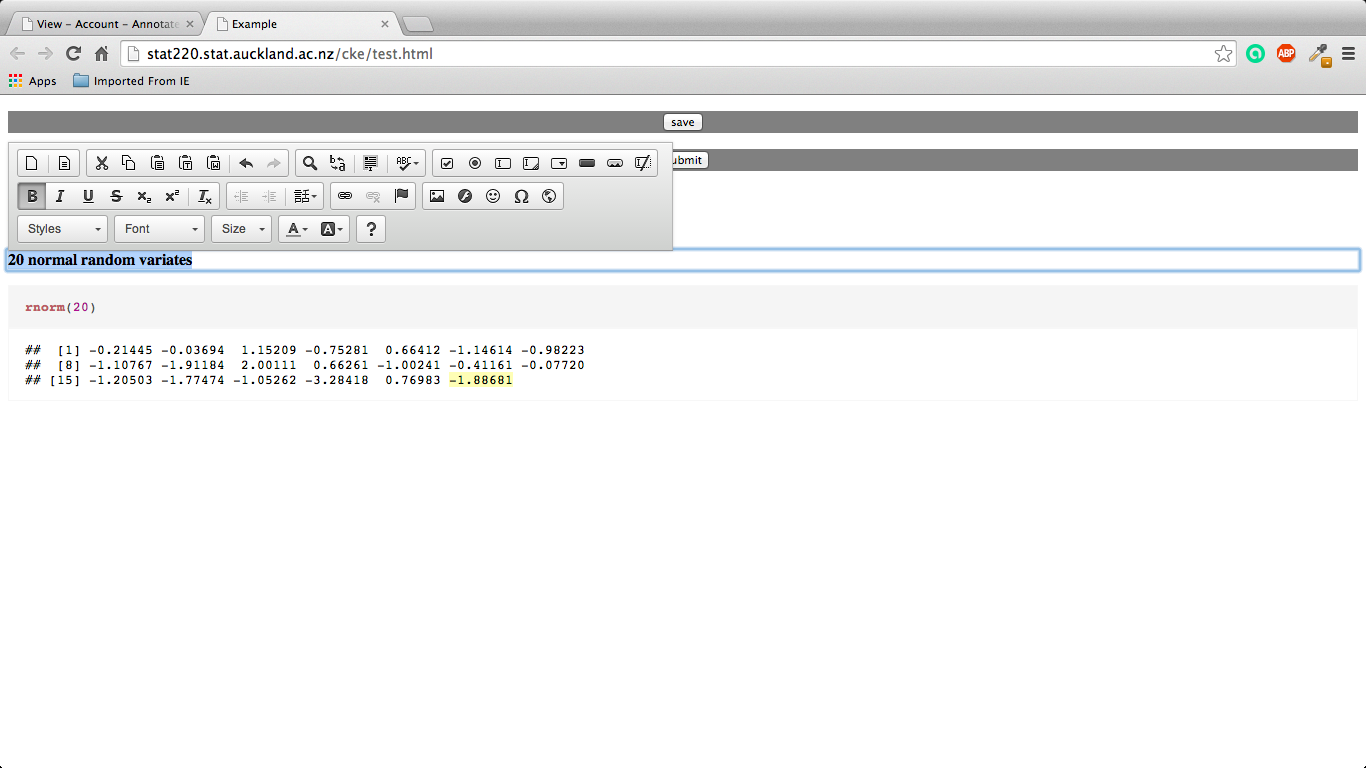
\includegraphics[trim=0cm 14cm 3cm 3.5cm,clip=true,width=1\textwidth,center]{changes}
\caption{\textbf{CKEditor} GUI}
\label{fig:2.3}
\end{figure}

\begin{figure}[h]
\includegraphics[trim=0cm 14cm 3cm 3.5cm,clip=true,width=1\textwidth,center]{annotate}
\caption{\texttt{Annotator} GUI}
\label{fig:2.4}
\end{figure}

The annotation is saved on a plain text file, \texttt{test-annotations.txt}, in \textbf{JSON} \citep{json} format and the change is saved on \texttt{test-changes.txt} as simple text. The code structure of these two files can be seen in Listings \ref{lst:2.3} and \ref{lst:2.4}.

\begin{lstlisting}[numbers=none, caption={\texttt{test-annotations.txt}}, label={lst:2.3}]
[
  {
    "ranges":  [
    {
      "start":          "/div[1]/div[1]/pre[1]",
      "startOffset":     8,
      "end":            "/div[1]/div[1]/pre[1]",
      "endOffset":      13
      }
    ],
    "quote":"speed",
    "text":"needs units",
    "id":"61430634697899221413241555634"
  }
]
\end{lstlisting}

\begin{lstlisting}[numbers=none, caption={\texttt{test-changes.txt}}, label={lst:2.4}]
EDITOR Editor-1 NOT MODIFIED

EDITOR Editor-2:
<code>summary(cars)</code>
\end{lstlisting}

The output of \texttt{snap()} consists of one file, e.g., the editable final document with \texttt{.edit.html} suffix, converted from the input suffix, \texttt{post.html}. The editable document is, then, uploaded onto the test server where editing occurs.

When the editing is completed, cliking on the ``save" button creates the two files, \texttt{test-annotations.txt} and \texttt{test-changes.txt}, on the test server for downloading and retrieval by other means.

%------------------------------------------------------------------------------
\subsubsection*{\texttt{annotations()}}
The function merges annotations from \texttt{test-annotations.txt} into the final document. The R package, \textbf{jsonlite} \citep{jsonlite}, is the tool used to convert the JSON data (the annotations in \texttt{test-annotation.txt}) into an R object, so that they can be merged into the final document.

Since the R-created sections are restricted to be annotated only, i.e., clients are not allowed to edit them, they require manual adjustments. For this reason, annotations are merged as (HTML) paragraphs with highlighted text and are inserted at the top of their original locations (in the R-created sections), to ease the burden of looking for them and manual merging them afterwards.

The default suffix of the output file is \texttt{.anns.html}, converted from the input suffix, \texttt{.edit.html}.

Listing \ref{lst:2.5} is the code structure of the final document merged with the annotation. The highlighted text, lines 10--12, displays the merged annotation.
\begin{lstlisting}[caption={(tidied) \texttt{example1.anns.html}}, escapechar=\|, label={lst:2.5}]
<!DOCTYPE html>
<html>
<head></head>
  <body>
    <p id="savebutton" style="background-color:grey; text-align:center">
      <button onclick="savechanges()">save</button>
    </p>
    <h1 contenteditable="true" id="Editor-1">Example</h1>
    <p contenteditable="true" id="Editor-2">Summary of the cars data:</p>
    |\hl{c}{<p class="annotation" style = "background-color:coral">}|
    |\hl{c}{<em>Annotation: The text "speed" was annotated with the}|
    |\hl{c}{message "needs units"</em></p>}|
    <div class="chunk" id="unnamed-chunk-1">
      <div class="rcode">
      <div class="output">
        <pre class="knitr r">
          ##      speed           dist    
          ##  Min.   : 4.0   Min.   :  2  
          ##  1st Qu.:12.0   1st Qu.: 26  
          ##  Median :15.0   Median : 36  
          ##  Mean   :15.4   Mean   : 43  
          ##  3rd Qu.:19.0   3rd Qu.: 56  
          ##  Max.   :25.0   Max.   :120
        </pre></div>
      </div></div>
  </body>
</html>
\end{lstlisting}


%------------------------------------------------------------------------------
\subsubsection*{\texttt{changes()}}
The function merges \emph{changes} in the file, \texttt{test-changes.txt}, into the final document.

The \emph{old} content, that has been edited, is replaced by the \emph{new} content, in \texttt{test-changes.txt}.

The default suffix of the output file is \texttt{.save.html}, converted from the input suffix, \texttt{.anns.html}.

Listing \ref{lst:2.6} is the code structure of the final document merged with the change. The highlighted text, line 10, shows the modified text.
\begin{lstlisting}[caption={(tidied) \texttt{example1.save.html}}, escapechar=\|, label={lst:2.6}]
<!DOCTYPE html>
<html>
<head></head>
  <body>
    <p id="savebutton" style="background-color:grey; text-align:center">
      <button onclick="savechanges()">save</button>
    </p>
    <h1 contenteditable="true" id="Editor-1">Example</h1>
    <p contenteditable="true" id="Editor-2">
|\hl{c}{<code>summary(cars)</code>}|
    </p>
    <p class="annotation" style = "background-color:coral">
    <em>Annotation: The text "speed" was annotated with the
    message "needs units"</em></p>
    <div class="chunk" id="unnamed-chunk-1">
      <div class="rcode">
      <div class="output">
        <pre class="knitr r">
          ##      speed           dist    
          ##  Min.   : 4.0   Min.   :  2  
          ##  1st Qu.:12.0   1st Qu.: 26  
          ##  Median :15.0   Median : 36  
          ##  Mean   :15.4   Mean   : 43  
          ##  3rd Qu.:19.0   3rd Qu.: 56  
          ##  Max.   :25.0   Max.   :120
        </pre></div>
      </div></div>
  </body>
</html>
\end{lstlisting}

Figure \ref{fig:2.5} shows how the \emph{annotated} and \emph{changed} final document, \texttt{example1.save.html} looks like in a web browser.
\begin{figure}[h]
\includegraphics[trim=0cm 20.4cm 0cm 1.8cm,clip=true,width=1\textwidth,center]{example1-save}
\caption{\texttt{example1.save.html}}
\label{fig:2.5}
\end{figure}


%------------------------------------------------------------------------------
\subsubsection*{\texttt{rip()}}
The function inverts final HTML-based documents, merged with changes and annotations, back into R HTML-based source documents.

More specifically, all unwanted contents added from the previous steps are removed. These include; the \texttt{script} and \texttt{style} elements added by \texttt{knit()} and \texttt{snap()}, the HTML attributes added by \texttt{snap()} and all R-created sections from \texttt{knit()}. The copies of R Code Chunks are reverted back to their original R HTML syntax, in place of the removed R-created sections, to become reproducible.

The default suffix of the output file is \texttt{.return.Rhtml}, converted from the input suffix, \texttt{.save.html}.

Listing \ref{lst:2.7} is the code structure of the inverted document, \texttt{example1.return.Rhtml}.
\begin{lstlisting}[caption={\texttt{example1.return.Rhtml}}, escapechar=\|, label={lst:2.7}]
<!DOCTYPE html>
<html>
<head>
</head>
  <body>
    <h1>Example</h1>
    <p>
<code>summary(cars)</code>
    </p>
    <p class="annotation" style = "background-color:coral">
    <em>Annotation: The text "speed" was annotated with the message "needs units"</em>
    <!--begin.rcode echo=FALSE
    summary(cars)
    end.rcode-->
  </body>
</html>
\end{lstlisting}

Rather than manually comparing the original source and inverted documents, we can use \texttt{diff} utility in UNIX system. The command line below is to compare the original source file, \texttt{example1.Rhtml} and the inverted source file, \texttt{example1.return.Rhtml}:
\begin{lstlisting}[numbers=none, frame=none]
$ diff example1.Rhtml example1.return.Rhtml
\end{lstlisting}

Listing \ref{lst:2.8} is the output from the previous \texttt{diff} command. It says line 7 of the original source document (Listing \ref{lst:2.1}) is changed with the lines 7--11 of the inverted file (Listing \ref{lst:2.7}).
\begin{lstlisting}[caption={Output from \texttt{diff}}, label={lst:2.8}]
7c7,11
<     <p>Summary of the cars data:</p>
---
>     <p>
> <code>summary(cars)</code>
>     </p>
>     <p class="annotation" style = "background-color:coral">
>     <em>Annotation: The text "speed" was annotated with the message "needs units"</em>
\end{lstlisting}



% There have been various ideas to support the logic behind the algorithms involved in the steps of the round trip. It is absolutely vital to explore deeper into each function for us to gain better understanding. The main purpose of this section is to simply discuss the role of each function in more detail in order to obtain adequate understanding of the overall project and hopefully answer any questions and uncertainties raised in the previous section.
% 
% \subsection{\texttt{sew()}}
% \label{subsec:1}
% One of the most important ideas to constantly remind ourselves was the preservation of the original R code. As briefly mentioned in Section \ref{sec:overview}, retaining the exactly identical R code (that we started with) is a fundamentally important aspect of the round trip in order to reproduce the identical source document. We have figured that the task of preserving the original R code would be much more difficult once the code is converted by the function \texttt{knit()}, as it would then require an extra step of text-processing on the converted R code. Gathering the original information from the converted format is unnecessary complication that we can avoid, which led us to a conclusion that the preservation should happen prior to the conversion step of \texttt{knit()}.
% 
% A possible solution is to formulate a similar strategy that the package \textbf{knitr} uses. As a reminder we can refer back to Listing \ref{lst:1} and note the way R code is presented. The original line of R code is wrapped inside slightly modified HTML comment tags (lines 9 and 11) which act as a marker to signal that the contents in these comments are intended to be displayed in the final document. In other words, the function \texttt{knit()} recognises these specific types of HTML comments and convert their contents (lines of R code) appropriately for display. The package requires the user to enclose all R code chunks intended for display in final documents in this special manner.
% 
% We have decided to implement a similar algorithm involving HTML comment tags through which the retention of the original R code is possible. The only conceptual difference between the two algorithms is in their objectives: detection of R code chunks for conversion in \textbf{knitr} and for preservation in ours. The algorithm we have formulated is to copy the original chunks of R code and insert the copies below the originals. In addition, the HTML comment tags to contain the copies are further modified so that they are explicitly controllable in later steps while avoiding detection from \texttt{knit()}. These copies remain technically as comments in the HTML syntax which can only be examined through the internal code structure of the document (hidden from display through a browser). As a result, the copies of R code chunks (generated by \texttt{sew()}) are preserved in all steps unless we decide to control them to undergo modification.
% 
% In summary, our function \texttt{sew()}:
% \begin{itemize}
%  \item detects any R code chunks that obey the required syntax of \textbf{knitr}, that is the chunks intended to be displayed in final documents, \\[-3ex]
%   \item creates identical copies of those (original) R code chunks with altered the comment tags and \\[-3ex]
%   \item inserts the copies below the corresponding R code chunks.
% \end{itemize}
% 
% The following command in R calls \texttt{sew()} on \texttt{example1.Rhml} to generate \texttt{example1.post.Rhtml}.
% 
% <<eval=FALSE>>=
% source("sew.R")
% sew("example1.Rhtml")
% @
% 
% Listing \ref{lst:3} shows the structure of the output document \texttt{example1.post.Rhtml} from \texttt{sew()}. Note that the code structures of the input document \texttt{example1.Rhtml} (Listing \ref{lst:1}) and the output document \texttt{example1.post.Rhtml} (Listing \ref{lst:3}) are identical except the highlighted text which represents the copy of the original R code (lines 9--11).
% 
% \begin{lstlisting}[caption={\texttt{example1.post.Rhml}}, escapechar=\|, label={lst:3}]
% <!DOCTYPE html>
% <html>
%   <head>
%     <title>Example</title>
%   </head>
%   <body>
%     <h1>Example</h1>
%     <p>20 random variates from the standard normal distribution</p>
%     <!--begin.rcode
%     rnorm(20)
%     end.rcode-->
%     |\hl{c}{<!--begin.keepcode}|
%     |\hl{c}{rnorm(20)}|
%     |\hl{c}{end.keepcode-->}|
%   </body>
% </html>
% \end{lstlisting}
% %------------------------------------------------------------------------------
% \subsubsection{\texttt{knit()}}
% \label{subsubsec:1}
% 
% The output document \texttt{example1.post.Rhtml} from the function \texttt{sew()} is ready to undergo the knitting procedure in a sense that the resultant document \texttt{example1.post.html} (from \texttt{knit()}) will always retain the original R code.
% 
% The following code is executed in R to knit the input document \texttt{example1.post.Rhtml}...
% <<eval=FALSE>>=
% knit("example1.post.Rhtml")
% @
% ...to generate the output document \texttt{example1.post.html} whose internal code structure can be examined in Listing \ref{lst:4}. Note that the highlighted lines represent that the copy of the original R code chunk which remains untouched by the knitting procedure.
% 
% \begin{lstlisting}[caption={\texttt{example1.post.Rhml}}, escapechar=\|, label={lst:4}]
% <!DOCTYPE html>
% <html>
%   <head>
%     |\emph{...lines of style from knitr}|
%     <title>Example</title>
%   </head>
%   <body>
%     <h1>Example</h1>
%     <p>20 random variates from the standard normal distribution</p>
% <div class="chunk" id="unnamed-chunk-1"><div class="rcode"><div class="source"><pre class="knitr r"><span class="hl kwd">rnorm</span><span class="hl std">(</span><span class="hl num">20</span><span class="hl std">)</span>
% </pre></div>
% <div class="output"><pre class="knitr r">##  [1]  0.21997 -1.02766  1.22804  0.78368 -0.09822 -1.41733  0.25276
% ##  [8] -0.89354  0.01876  2.55360 -0.46999  1.14496  0.57621 -0.12584
% ## [15] -0.40660 -1.74065  0.27885  0.90726 -0.97394  0.62497
% </pre></div>
% </div></div>
% 
%     |\hl{c}{<!--begin.keepcode}|
%     |\hl{c}{rnorm(20)}|
%     |\hl{c}{end.rcode-->}|
%   </body>
% </html>
% \end{lstlisting}
% 
% Figure \ref{fig:4} shows how the document \texttt{example1.post.html} looks like in a browser. We should notice that the copy of the origiinal R code is hidden from the display and the only differences in the browser-display are the random variates.
% 
% \begin{figure}[h]
% 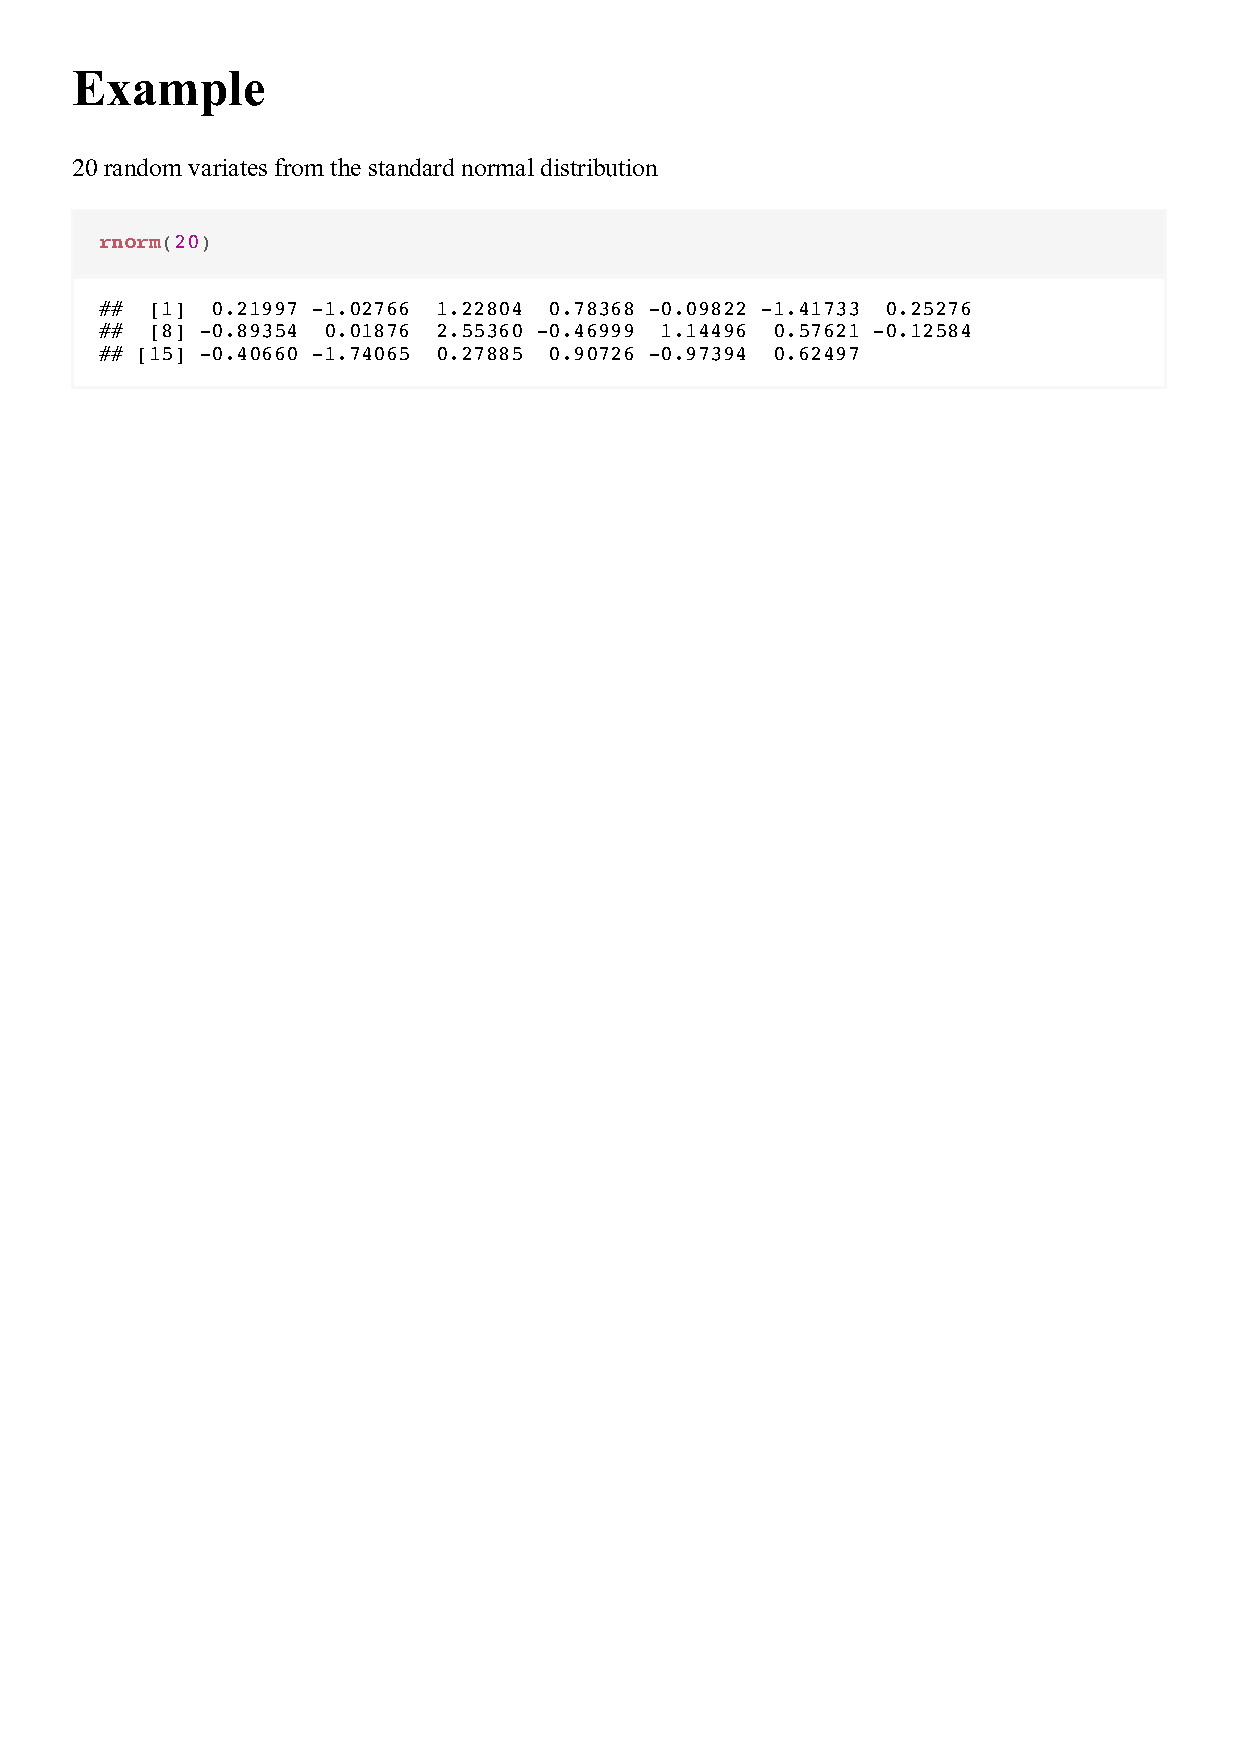
\includegraphics[trim=0cm 23cm 0cm 0cm,clip=true,width=1.1\textwidth,center]{example1_post}
% \caption{\texttt{example1.post.html} in a browser}
% \label{fig:4}
% \end{figure}
% 
% %------------------------------------------------------------------------------
% \pagebreak
% \subsection{\texttt{snap()}}
% \label{subsec:2}
% So far, we have managed to come up with a way to execute the function \texttt{knit()} on source documents (\texttt{.Rhtml}) while preserving the original information of R code chunks. The next stage of the round trip reflects on our primary objective (of the project), that is to be able to directly edit HTML documents that \texttt{knit()} produces. Possible complications involving the restriction due to \textbf{knitr}'s unidirectional document generation (Section \ref{ch:motiv}) have led us to a decision to implement the use of annotations. Especially the sections of R-related contents in final documentation are considered pointless to be directly edited as it will only result in text-based modification and will not have any impact on generating new results from the modified code. To gain the conceptual benefits of editing as discussed in Section \ref{ch:motiv}, these sections of R-associated contents are decided to be annotated to effectively deliver necessary messages from a person (editor) to another (viewer).
% 
% The first task of the function \texttt{snap()} is designed to identify the parts of an input document that should be editable. The editable sections are identified by searching for all top level elements inside the HTML body of the input document that are not introduced by the function \texttt{knit()}. Then two special attributes are inserted into the opening tag of each of these identified, editable elements: one to serve as a marker to let us know the corresponding element is editable and the other to ``number" the editable elements so that we can deal with them in an orderly manner in later steps. The top elements of annotatable sections (the R-associated contents) are identified by their distict attributes defined by \textbf{knitr}.
% After correctly identifying and marking up all the editable elements, the input document is appended with two supplementary sections of code, namely \texttt{button.html} and \texttt{edit.js}. The HTML code piece \texttt{button.html} contains definition of the designs for two HTML buttons called \texttt{save} and \texttt{submit} while the JavaScript code piece \texttt{edit.js} includes a few assigned instructions. Firstly, \texttt{edit.js} loads the \textbf{jQuery} library and two JavaScript modules named \textbf{CKEditor} and \textbf{AnnotateIt} whose respective functions are to enable browser-based editing and annotating on HTML documentation. Secondly, \texttt{edit.js} is instructed with the actions for the \texttt{save} button, which is to save any changes and annotations made via \textbf{CKEditor} and \textbf{AnnotateIt} as separate text files on a server, and for the \texttt{submit} button, which is to re-direct the browser to an uploading web page on the server (which will be discussed shortly) as well as saving the changes and annotations.
% 
% Once the input document is merged with the contents of \texttt{button.html} and \texttt{edit.js}, an \texttt{.edit.html} document is generated as the output of the function \texttt{snap()}. The resulting \texttt{.edit.html} document is then uploaded onto our test server through which the actual editing and annotating of the document occur. If we refer back to Listing \ref{lst:4}, the lines 10, 11 and 12 are the three top level elements inside the body of the HTML document. By our definition, the first two elements (lines 10 and 11), which correspond respectively to a (most important) heading and a paragraph, are editable and the third element (line 12), characterised by the attribute \texttt{class="chunk"} as an element added by \textbf{knitr}, is annotatable.
% 
% The following code is used in R to call the function \texttt{snap()} on the input document \texttt{example1.post.html} to generate the output document \texttt{example1.edit.html}.
% 
% <<eval=FALSE>>=
% source("snap.R")
% snap("example1.post.html")
% @
% 
% Listing \ref{lst:5} exhibits the internal code structure of the output document. The highlighted text (lines 10 and 11) shows the attributes added by the function \texttt{snap()}. Note that the first attributes \texttt{contenteditable="true"} are used to let \texttt{snap()} recognise the corresponding elements as editable and the second \texttt{id="Editor"} attributes are used to mark up the elements in a sequential manner.
% 
% \begin{lstlisting}[caption={\texttt{example1.edit.html}}, escapechar=\|, label={lst:5}]
% <!DOCTYPE html>
% <html>
%   <head>
%     |\emph{...lines of edit.js...}|
%     |\emph{...lines of style from knitr...}|
%     <title>Example</title>
%   </head>
%   <body>
%     |\emph{...lines of button.html...}|
%     <h1 |\hl{c}{contenteditable="true"}| |\hl{c}{id="Editor-1"}|>Example</h1>
%     <p |\hl{c}{contenteditable="true"}| |\hl{c}{id="Editor-2"}|>20 random variates from the standard normal distribution</p>
% <div class="chunk" id="unnamed-chunk-1"><div class="rcode"><div class="source"><pre class="knitr r"><span class="hl kwd">rnorm</span><span class="hl std">(</span><span class="hl num">20</span><span class="hl std">)</span>
% </pre></div>
% <div class="output"><pre class="knitr r">##  [1]  0.21997 -1.02766  1.22804  0.78368 -0.09822 -1.41733  0.25276
% ##  [8] -0.89354  0.01876  2.55360 -0.46999  1.14496  0.57621 -0.12584
% ## [15] -0.40660 -1.74065  0.27885  0.90726 -0.97394  0.62497
% </pre></div>
% </div></div>
% 
%     <!--begin.keepcode
%     rnorm(20)
%     end.keepcode-->
%   </body>
% </html>
% \end{lstlisting}
% 
% The \texttt{.edit.html} document is then uploaded on to the test server. The browser-display of the document, on the server, can be seen in Figure \ref{fig:5} where the top and bottom displays represent the editable and annotatable environments of \textbf{CKEditor} and \textbf{AnnotateIt} respectively. Editing occurs by each element, that is each section (of the element) must be clicked separately to bring up the editable environment. Attaching annotations requires the user to have an account with \textbf{AnnotateIt} and be logged into their website \url{http://annotateit.org/}. In addition, annotations are made on selections of text of the annotatable sections. Notice the \texttt{save} and \texttt{submit} buttons at the top of the display which can be clicked to save the changes and annotations made. It is of great importance to keep in mind that the execution of editing and annotating takes place simultaneously on the uploaded document to create two separate save files with the information on the annotations and the text-based changes when the \texttt{save} or \texttt{submit} button is clicked.
% 
% \begin{figure}[h]
% 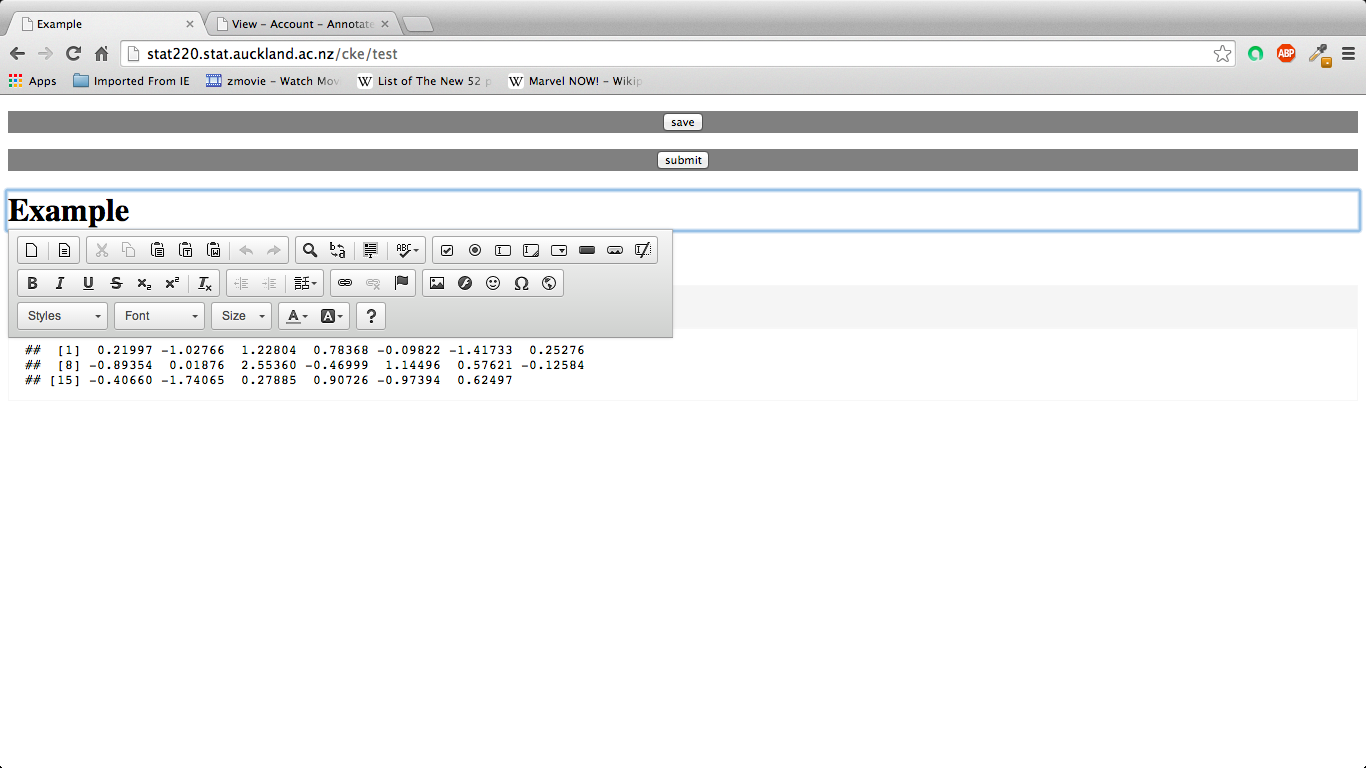
\includegraphics[trim=0cm 9cm 0cm 3.5cm,clip=true,width=1\textwidth,center]{CKEditor}
% 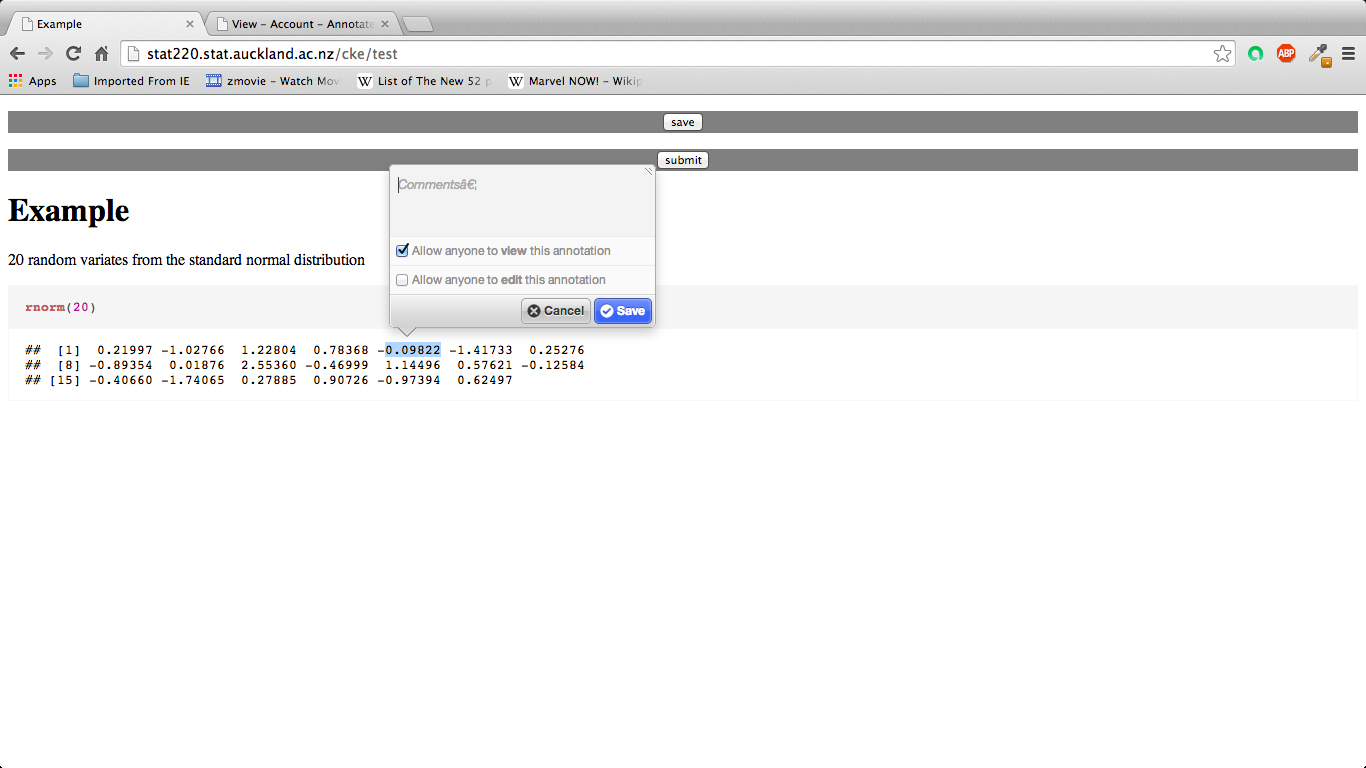
\includegraphics[trim=0cm 11.5cm 0cm 3.5cm,clip=true,width=1\textwidth,center]{AnnotateIt}
% \caption{\texttt{example1.edit.html}, uploaded on the server, in a browser}
% \label{fig:5}
% \end{figure}
% 
% In summary, the function \texttt{snap()}:
% \begin{itemize}
%  \item identifies and marks up all editable top level elements, present in input documents, in a sequential manner, \\[-3ex]
%  \item appends the two supplementary sections of code \texttt{buttons.html} and \texttt{edit.js} into the input documents whose respective purposes are: \\[-3ex]
%  %
%  \begin{enumerate}[i]
%   \item the provision of the designs for the two \texttt{save} and \texttt{submit} buttons and \\[-3ex]
%   \item to load the \textbf{jQuery} library, enable \textbf{CKEditor} and \textbf{AnnotateIt} on editable and annotatable sections of the input documents respectively, and save the changes and annotations made through the two JavaScript modules as text files on the test server when the buttons are clicked, with an additional feature of re-directing the browser to the uploading web page when the \texttt{submit} button is clicked, and
%  \end{enumerate}
%  %
%  \item finally generate \texttt{.edit.html} documents as the output which can then be uploaded onto the server for the actual editing and annotating of the documents to take place.
% \end{itemize}
% 
% %------------------------------------------------------------------------------
% \subsection{\texttt{annotations()}}
% \label{subsec:3}
% The information on annotations made via the JavaScript module \texttt{AnnotateIt} is accessed from the test server as a text file. The module generates the save file in the JSON format for which we have decided to use an R package called \textbf{jsonlite} to effectively deal with the file format. The save file can be directly fetched from the server by using another R package \textbf{RCurl} and can then be processed, in the manner regarding the JSON format, to generate a message for each annotation. The most informative data such as the selection of text for annotations, the author of the annotations and the annotations themselves are extracted from the save file in order to generate the message.
% 
% Figure \ref{fig:6} is a minimal demonstration of creating an annotation. The last random variate is selected to be marked with the annotation ``Example". Upon clicking the blue \texttt{Save} button on the pop-up window, a save file is created by \textbf{AnnotateIt} on the test server.
% 
% \begin{figure}[h]
% 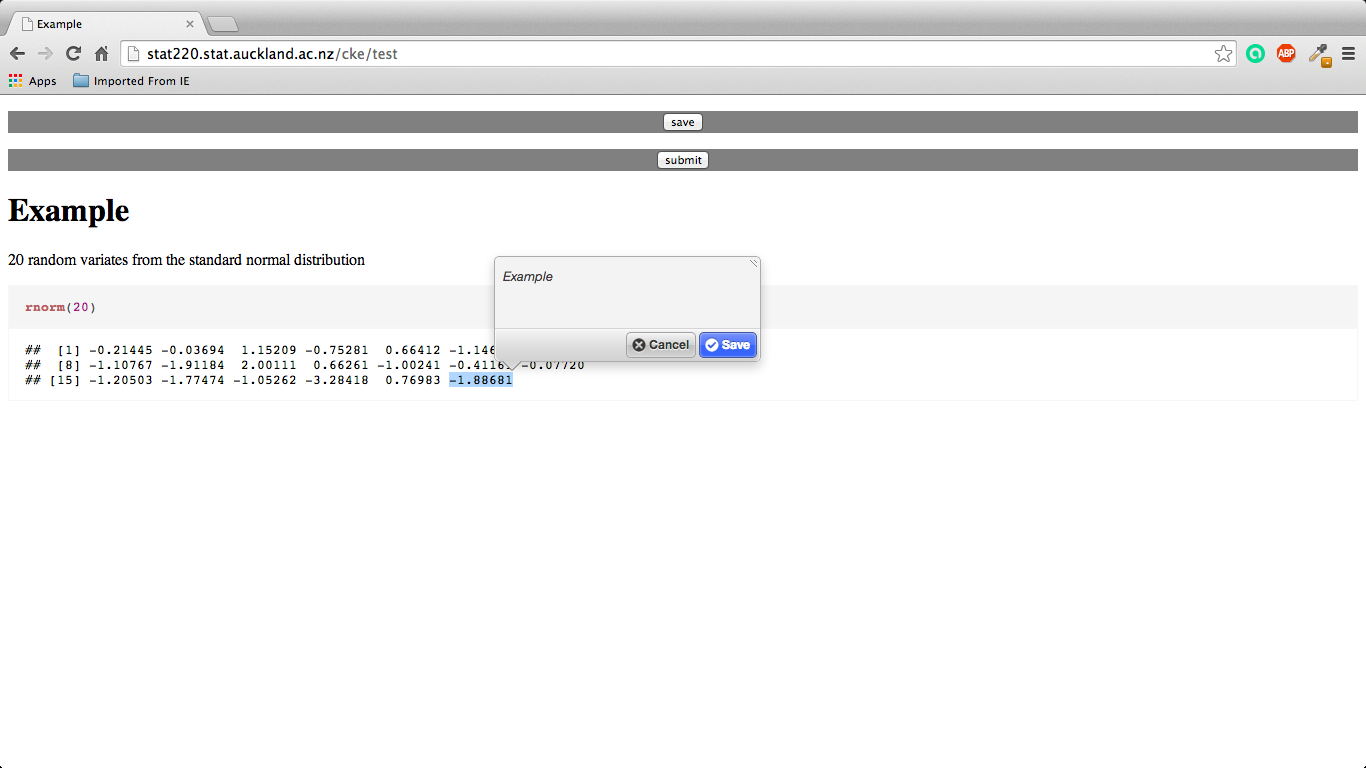
\includegraphics[trim=0cm 11.5cm 0cm 3.5cm,clip=true,width=1\textwidth,center]{annotations}
% \caption{annotating on \texttt{example1.edit.html}}
% \label{fig:6}
% \end{figure}
% 
% The following code is used in R to call the function \texttt{annotations()} on the input document \texttt{example1.edit.html} to generate the output document \texttt{example1.anns.html}.
% 
% <<eval=FALSE>>=
% source("annotations.R")
% annotations("example1.edit.html")
% @
% 
% Listing \ref{lst:6} is the internal code structure of the output document \texttt{example1.anns.html} where the highlighted lines of text (lines 12--14) represent the message genereated according to the information from the save file. The message is in a paragraph tag with the \texttt{class="annotation"} and its own style attributes.
% 
% \begin{lstlisting}[caption={\texttt{example1.anns.html}}, escapechar=\|, label={lst:6}]
% <!DOCTYPE html>
% <html>
%   <head>
%     |\emph{...lines of edit.js...}|
%     |\emph{...lines of style from knitr...}|
%     <title>Example</title>
%   </head>
%   <body>
%     |\emph{...lines of button.html}|
%     <h1 contenteditable="true" id="Editor-1">Example</h1>
%     <p contenteditable="true" id="Editor-2">20 random variates from the standard normal distribution</p>
% |\hl{c}{<p class="annotation" style = "background-color:coral">}|
% |\hl{c}{The text "-1.88681" was annotated with the message "Example" by "e.lim0322"}|
% |\hl{c}{</p>}|
% <div class="chunk" id="unnamed-chunk-1"><div class="rcode"><div class="source"><pre class="knitr r"><span class="hl kwd">rnorm</span><span class="hl std">(</span><span class="hl num">20</span><span class="hl std">)</span>
% </pre></div>
% <div class="output"><pre class="knitr r">##  [1] -0.21445 -0.03694  1.15209 -0.75281  0.66412 -1.14614 -0.98223
% ##  [8] -1.10767 -1.91184  2.00111  0.66261 -1.00241 -0.41161 -0.07720
% ## [15] -1.20503 -1.77474 -1.05262 -3.28418  0.76983 -1.88681
% </pre></div>
% </div></div>
% 
%     <!--begin.keepcode
%     rnorm(20)
%     end.keepcode-->
%   </body>
% </html>
% \end{lstlisting}
% 
% Figure \ref{fig:7} shows the document \texttt{example1.anns.html} in a browser. The text highlighted in red is the message.
% 
% \begin{figure}[h]
% 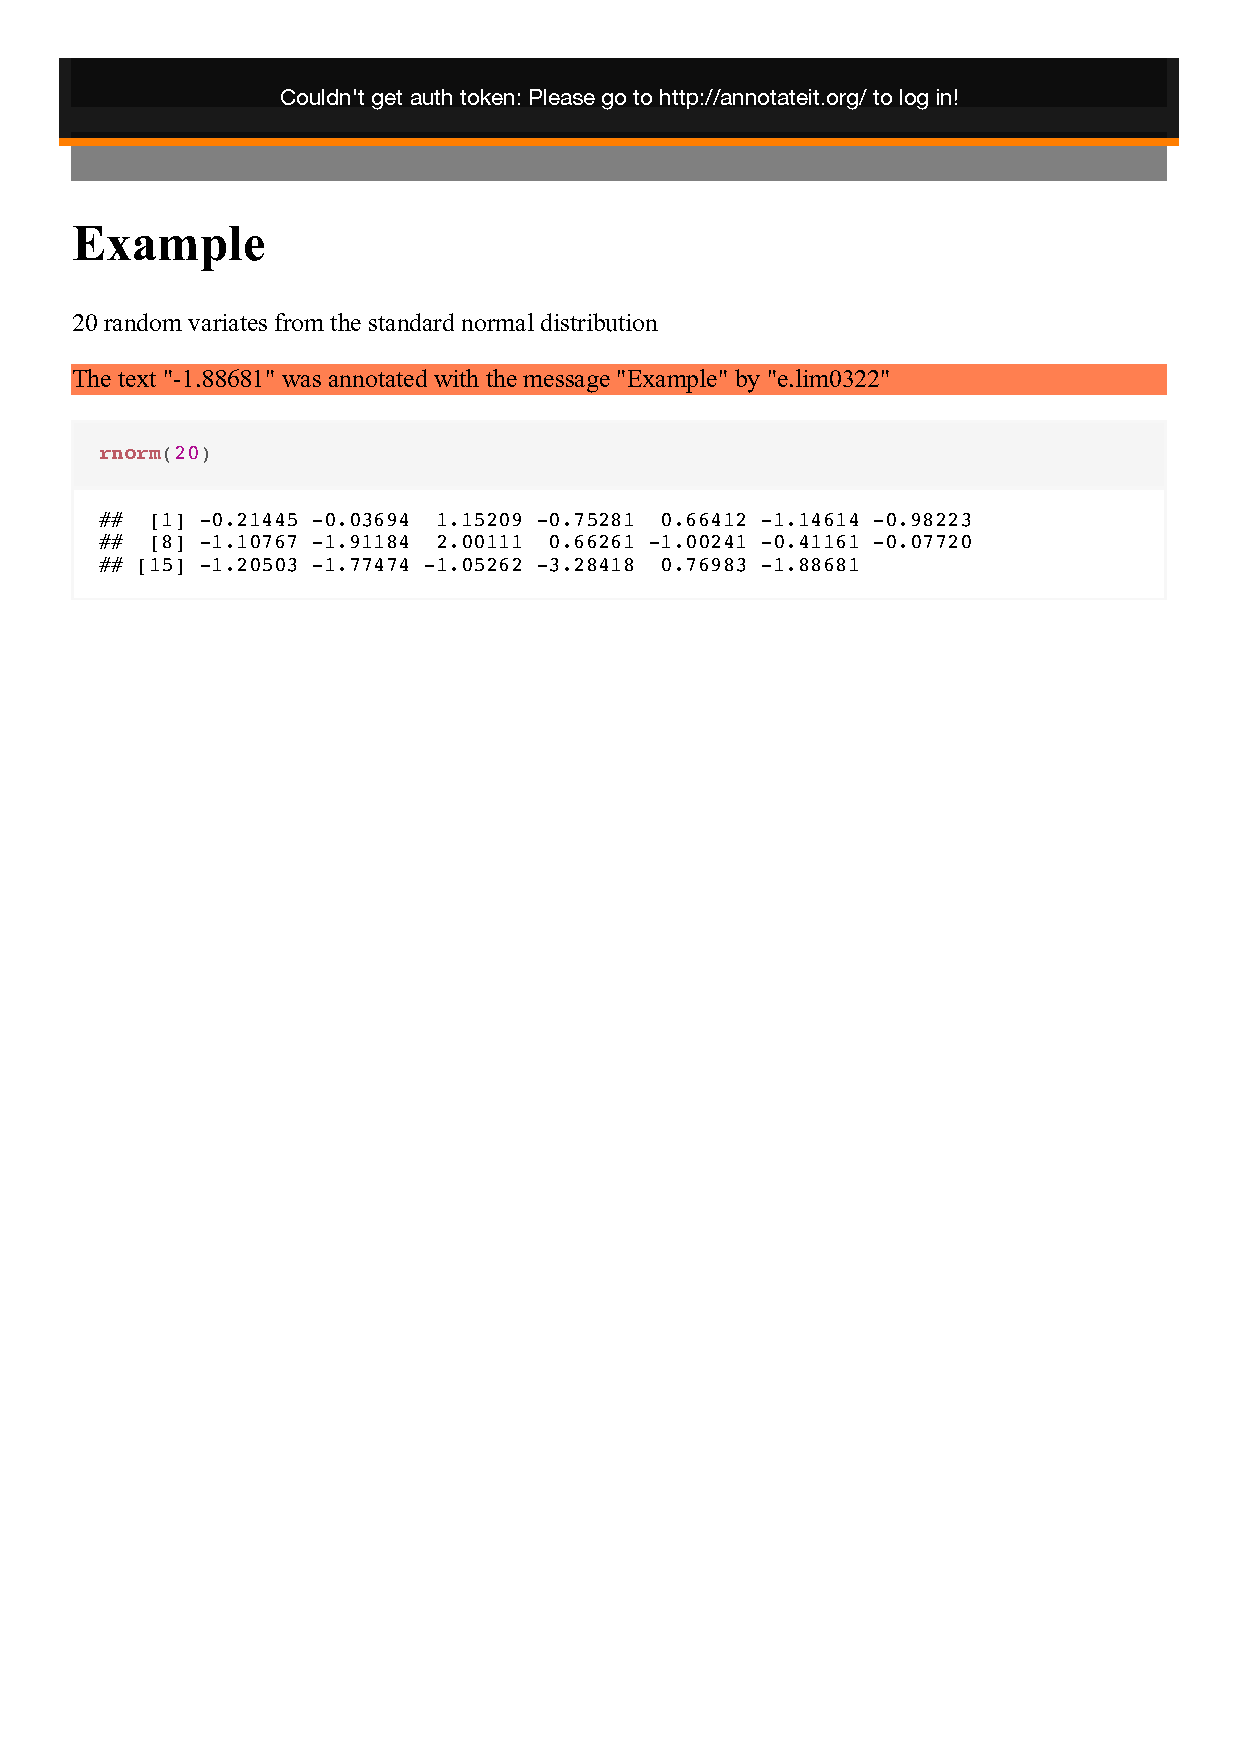
\includegraphics[trim=0cm 19.5cm 0cm 3.2cm,clip=true,width=1.1\textwidth,center]{example1_anns}
% \caption{\texttt{example1.anns.html} in a browser}
% \label{fig:7}
% \end{figure}
% 
% %------------------------------------------------------------------------------
% \subsection{\texttt{changes()}}
% \label{subsec:4}
% The primary task assigned to the function \texttt{changes()} is to access the save file for the changes made through \textbf{CKEditor} from the server and replace the old, modified text (in the input document) with the new text (in the save file). This replacement takes place only for the sections that are actually edited.
% 
% Figure \ref{fig:8} illustrates a brief demonstration of how the process of editing is carried out. The first editable section, which is the heading, is left as it is while the second editable section is chosen to be edited. The original line of text ``20 random variates from..." is to be edited with the bold faced text ``20 normal random variates". When the grey \texttt{save} button is clicked, the save file of the change is created on the server which is a simple text file with the code structure as shown in Listing \ref{lst:7}.
% 
% \begin{figure}[h]
% 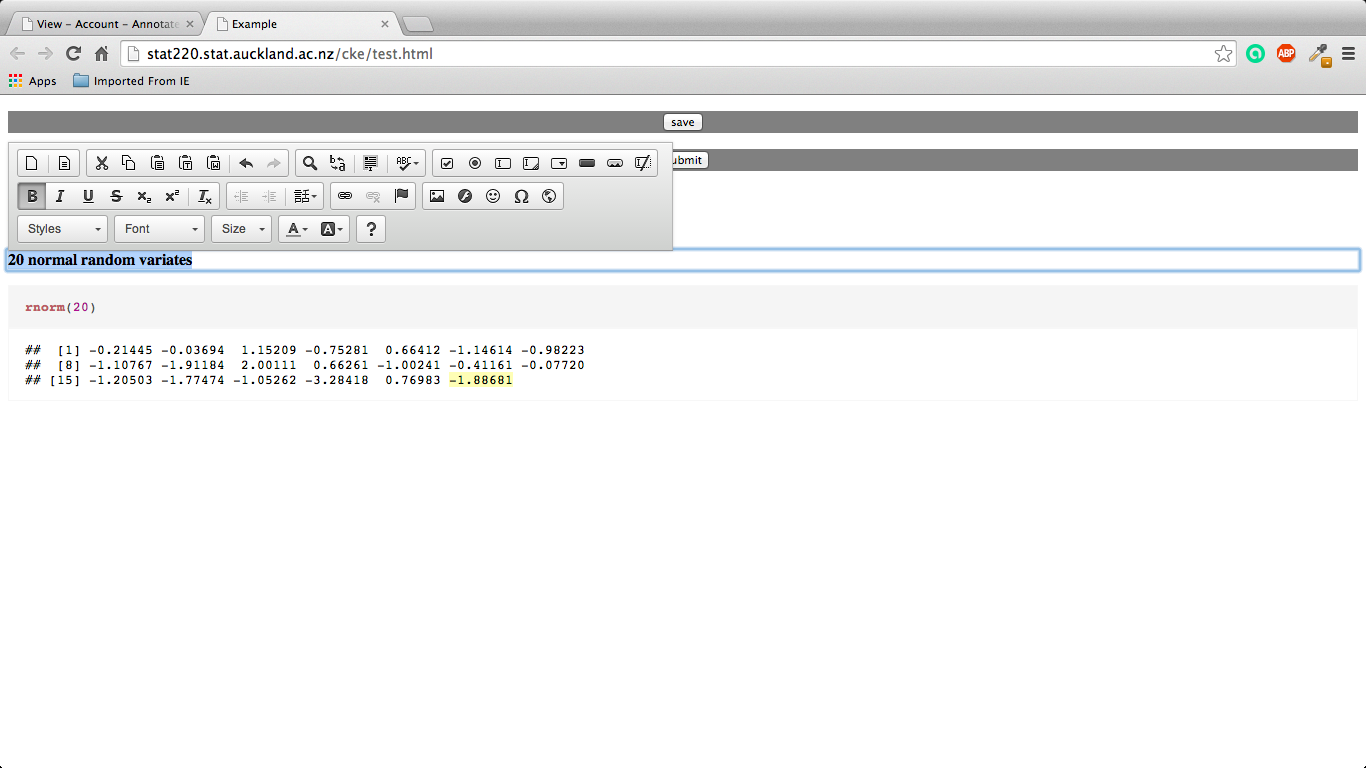
\includegraphics[trim=0cm 12cm 0cm 3.5cm,clip=true,width=1\textwidth,center]{changes}
% \caption{editing \texttt{example1.edit.html}}
% \label{fig:8}
% \end{figure}
% 
% Note the first line in Listing \ref{lst:7}. This line corresponds to the editable element (in \texttt{example1.edit.html}) with an attribute defined as \texttt{Editor-1}, that is the line 10 in Listing \ref{lst:5}, which is the heading. As we can see the heading is ``\texttt{NOT MODIFIED}" to allow the function \texttt{changes()} to ignore this editable section  of the document. On the other hand, the line 4 displays the desired change on the second editable section.
% 
% \begin{lstlisting}[caption={\texttt{changes.txt}}, escapechar=\|, label={lst:7}]
% EDITOR Editor-1 NOT MODIFIED
% 
% EDITOR Editor-2:
% <strong>20 normal random variates</strong>
% \end{lstlisting}
% 
% The following code is used in R to call the function \texttt{changes()} on the input document \texttt{example1.anns.html} to generate the output document \texttt{example1.save.html}.
% 
% <<eval=FALSE>>=
% source("changes.R")
% changes("example1.anns.html")
% @
% 
% The internal code structure of the output document \texttt{example1.save.html} can be seen in Listing \ref{lst:8}. The highlighted text (line 12) shows that the old line (line 11 in Listing \ref{lst:6}) is replaced with the change (line 4 in Listing \ref{lst:7}) by \texttt{snap()} to result in a display through a browser as shown in Figure \ref{fig:9}.
% 
% \begin{lstlisting}[caption={\texttt{example1.save.html}}, escapechar=\|, label={lst:8}]
% <!DOCTYPE html>
% <html>
%   <head>
%     |\emph{...lines of edit.js...}|
%     |\emph{...lines of style from knitr...}|
%     <title>Example</title>
%   </head>
%   <body>
%     |\emph{...lines of button.html}|
%     <h1 contenteditable="true" id="Editor-1">Example</h1>
%     <p contenteditable="true" id="Editor-2">
% |\hl{c}{<strong>20 normal random variates</strong>}|
%     </p>
%     <p class="annotation" style = "background-color:coral">
%     The text "-1.88681" was annotated with the message "Example" by "e.lim0322"
%     </p>
% <div class="chunk" id="unnamed-chunk-1"><div class="rcode"><div class="source"><pre class="knitr r"><span class="hl kwd">rnorm</span><span class="hl std">(</span><span class="hl num">20</span><span class="hl std">)</span>
% </pre></div>
% <div class="output"><pre class="knitr r">##  [1] -0.21445 -0.03694  1.15209 -0.75281  0.66412 -1.14614 -0.98223
% ##  [8] -1.10767 -1.91184  2.00111  0.66261 -1.00241 -0.41161 -0.07720
% ## [15] -1.20503 -1.77474 -1.05262 -3.28418  0.76983 -1.88681
% </pre></div>
% </div></div>
% 
%     <!--begin.keepcode
%     rnorm(20)
%     end.keepcode-->
%   </body>
% </html>
% \end{lstlisting}
% 
% The text is successfully edited in Figure \ref{fig:9}.
% 
% \begin{figure}[h]
% 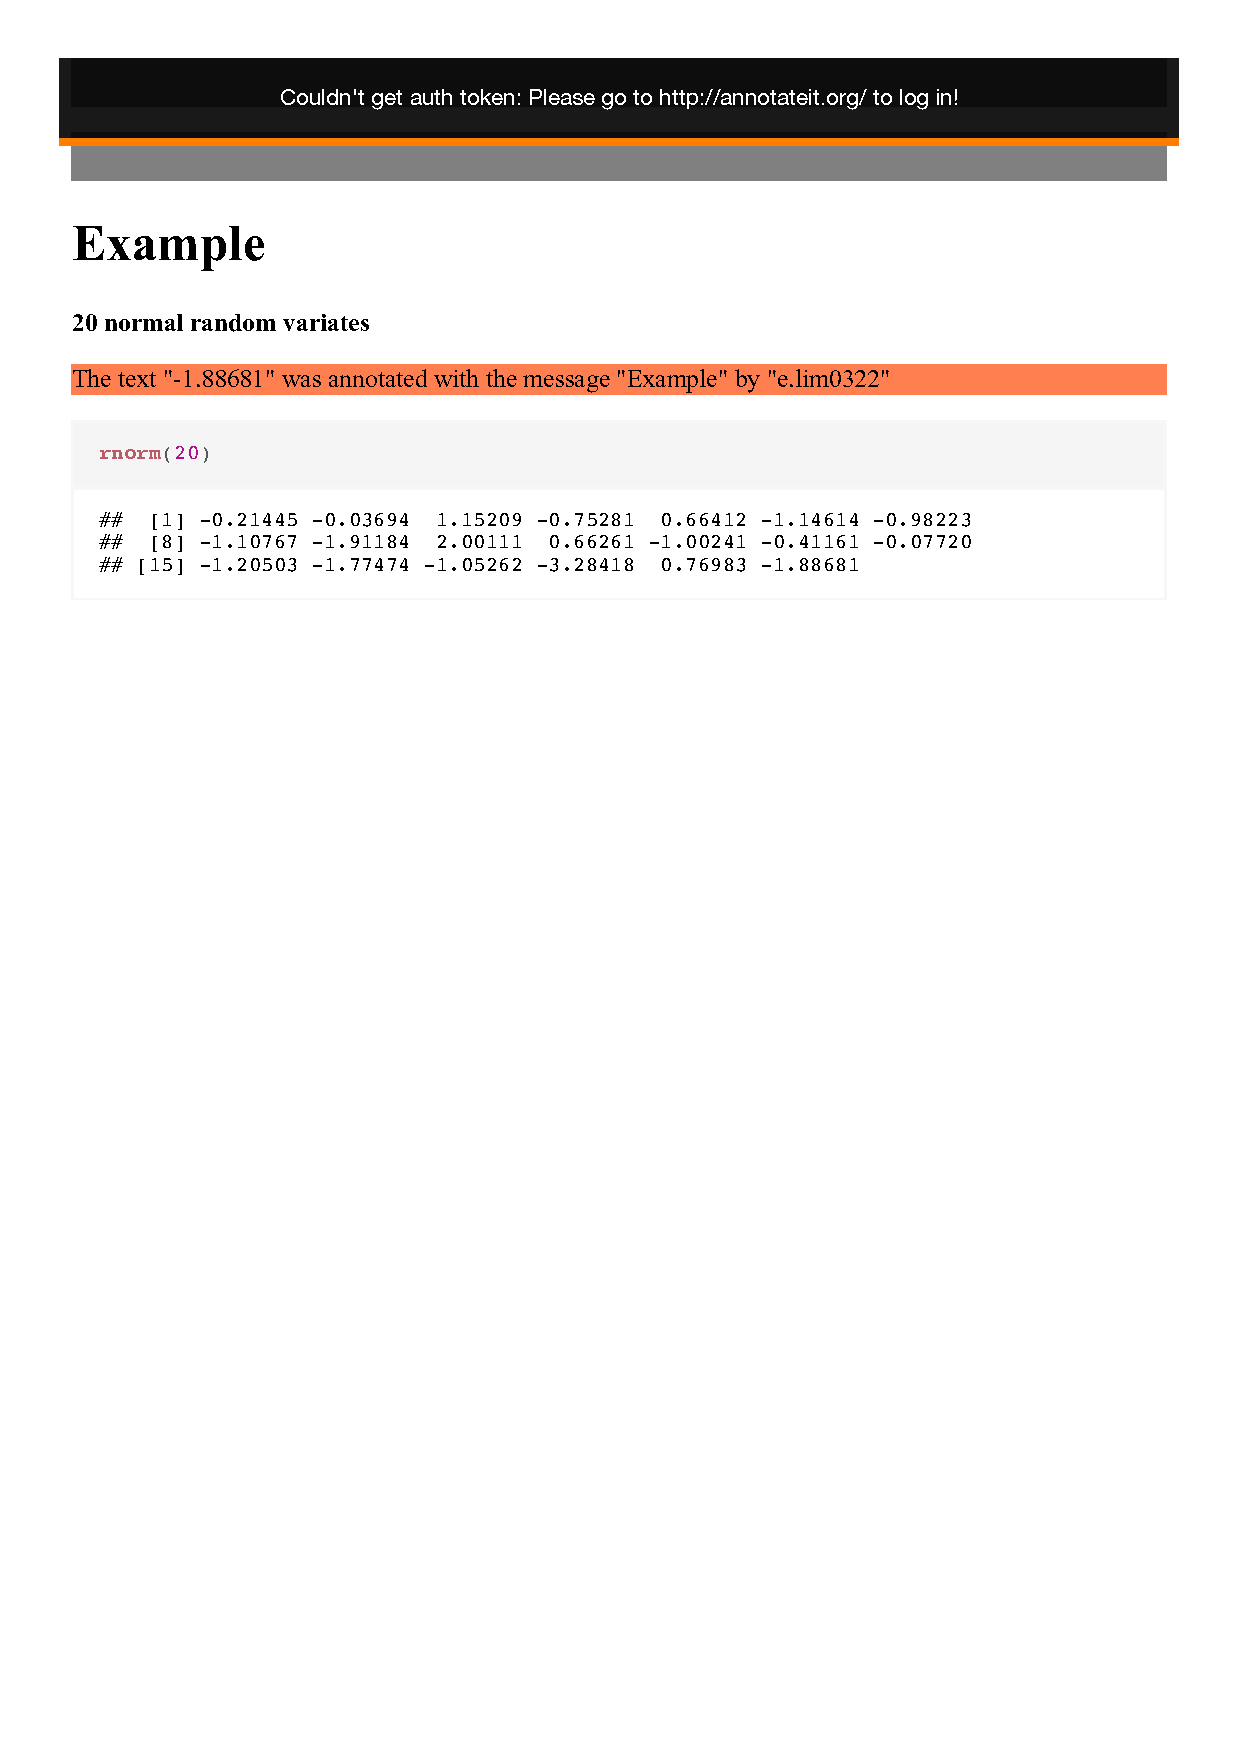
\includegraphics[trim=0cm 19.5cm 0cm 3.2cm,clip=true,width=1.1\textwidth,center]{example1_save}
% \caption{\texttt{example1.save.html} in a browser}
% \label{fig:9}
% \end{figure}
% 
% %------------------------------------------------------------------------------
% \subsection{\texttt{rip()}}
% \label{subsec:5}
% The main purpose of the function \texttt{rip()} is to return to the original source document format while retaining changes and annotations. It searches for any foreign lines of code that are introduced by \textbf{knitr} or inserted during certain stages of the round trip, and removes those lines. Typically, the lines of the CSS style inserted by \textbf{knitr} are removed first, followed by the lines corresponding to the \texttt{div} elements generated and inserted by \textbf{knitr} (e.g. lines 17--23 in Listing \ref{lst:8}). These \texttt{div} elements are defined with the attribute \texttt{class="chunk"} which can be identified by \texttt{snap()} to recognise them as the elements introduced by \textbf{knitr}. Then the copies of the original R code chunks (lines 12--14 in Listing \ref{lst:3}) are modified by \texttt{snap()} to be exactly as the originals. The text ``\texttt{keep}" in the comment tags of the copy (lines 12 and 14 in Listing \ref{lst:3}) are identified and converted to the letter ``\texttt{r}" so that both the opening and closing comment tags are like the originals. The lines of \texttt{button.html} and \texttt{edit.js} are also removed as well as the two attributes \texttt{contenteditable="true"} and \texttt{id="Editor"}, added to mark up the corresponding elements as editable (Section \ref{subsec:2}).
% 
% The following R code calls the function \texttt{rip()} on the input document \texttt{example1.save.html} to generate the output document \texttt{example1.return.Rhtml}.
% 
% <<eval=FALSE>>=
% source("rip.R")
% rip("example1.save.html")
% @
% 
% The internal code structure of the output document \texttt{example1.return.Rhtml} can be seen in Listing \ref{lst:9}. If we compare the code structure of the source document \texttt{example1.Rhtml} with that of \texttt{example1.return.Rhtml}, we can notice that line 8 in Listing \ref{lst:1} (original) is replaced by the edited text in line 9 of Listing \ref{lst:9}. Lines 11--13 in Listing \ref{lst:9} are the generated messages for the annotations from the previous step (Section \ref{subsec:3}). Apart from these lines, the rest of both documents are identical.
% 
% \begin{lstlisting}[caption={\texttt{example1.save.html}}, escapechar=\|, label={lst:9}]
% <!DOCTYPE html>
% <html>
%   <head>
%     <title>Example</title>
%   </head>
%   <body>
%     <h1>Example</h1>
%     <p>
% <strong>20 normal random variates</strong>
%     </p>
%     <p class="annotation" style = "background-color:coral">
%     The text "-1.88681" was annotated with the message "Example" by "e.lim0322"
%     </p>
%     <!--begin.rcode
%     rnorm(20)
%     end.keepcode-->
%   </body>
% </html>
% \end{lstlisting}
% 
% We can knit the ``final" source document \texttt{example1.return.Rhtml} by the following code in R.
% 
% <<eval=FALSE>>=
% knit("example1.return.Rhtml")
% @
% 
% The display of the knitted document \texttt{example1.return.html} through a browser can be seen in Figure \ref{fig:10}.
% 
% \begin{figure}[h]
% 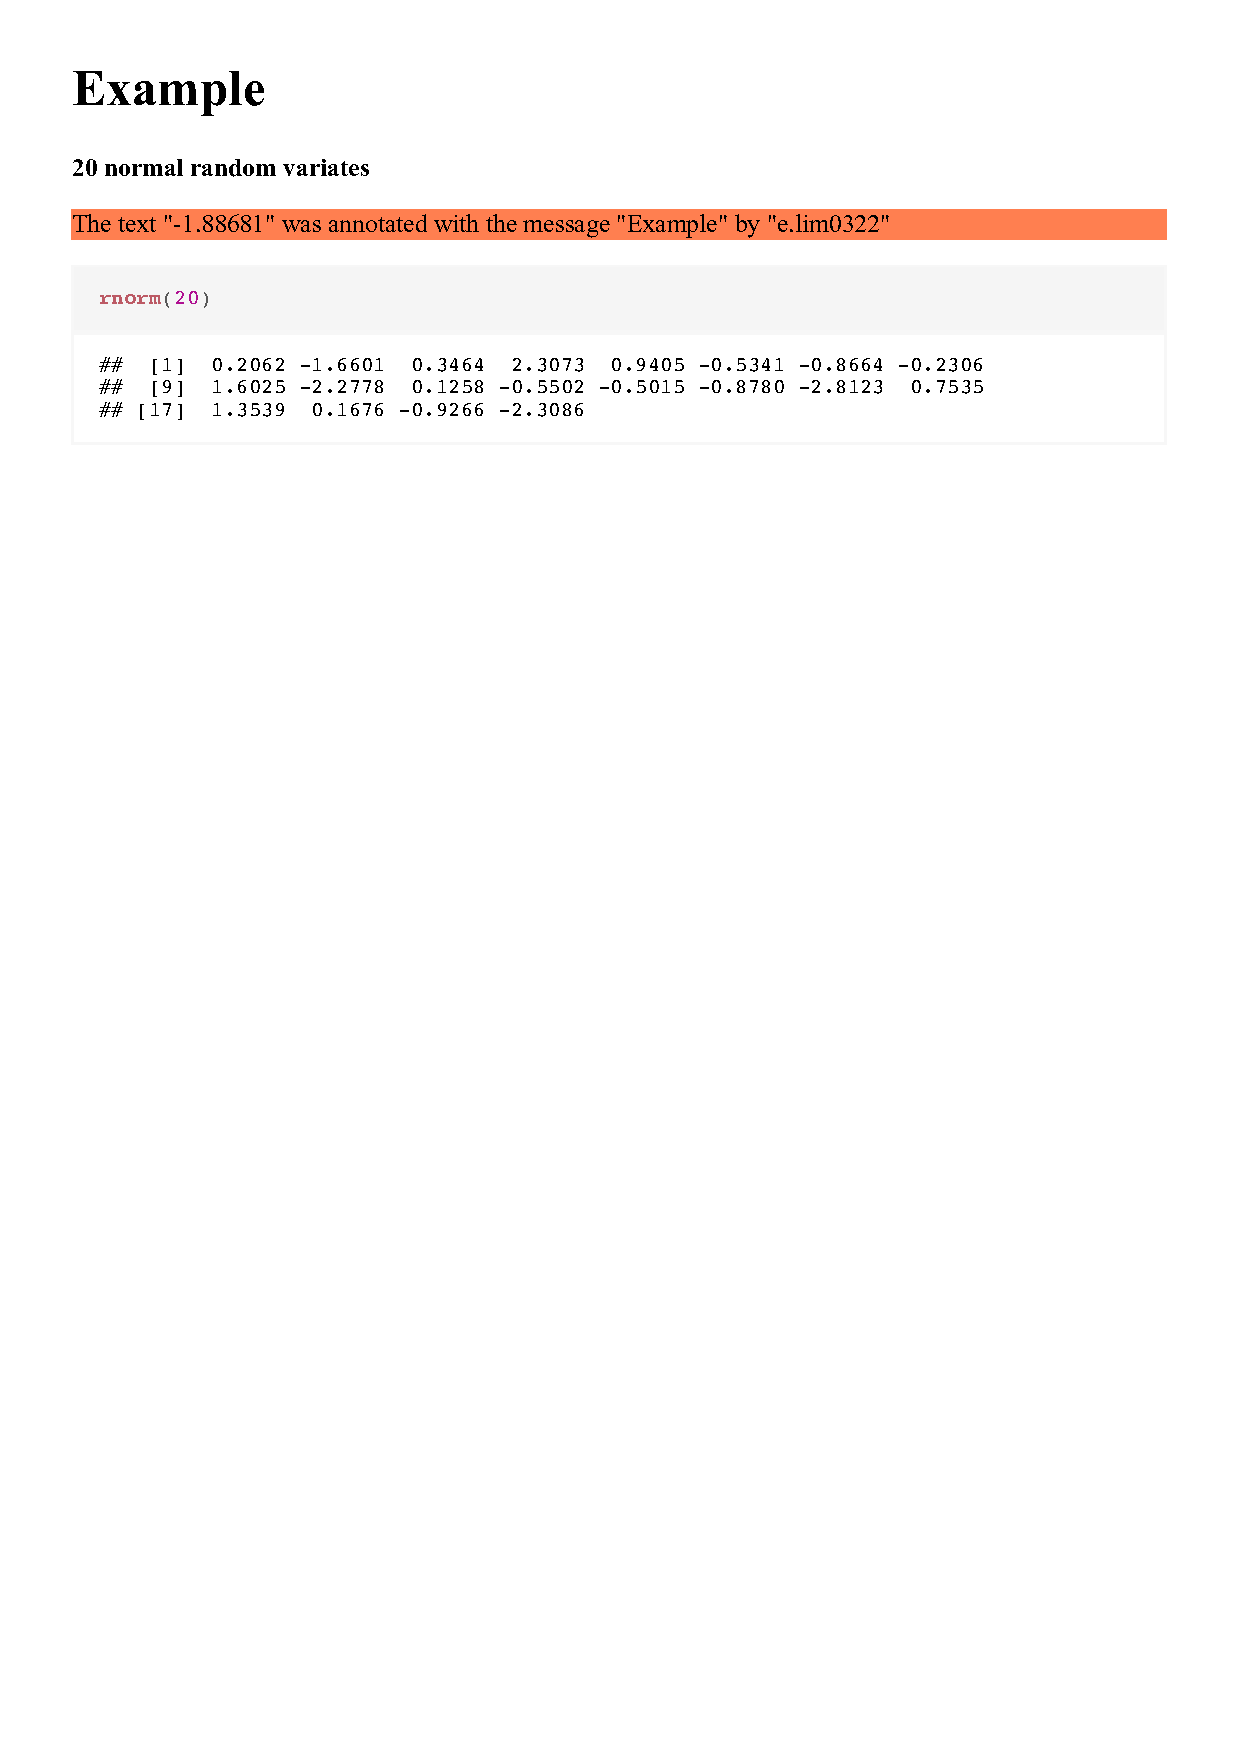
\includegraphics[trim=0cm 22cm 0cm 0cm,clip=true,width=1.1\textwidth,center]{example1_return}
% \caption{\texttt{example1.return.html} in a browser}
% \label{fig:10}
% \end{figure}
% 
% 
%


%------------------------------------------------------------------------------
%----------------------------- Phase 2: Markdown ------------------------------
%------------------------------------------------------------------------------
\chapter{Phase 2: R Markdown}
\begin{figure}[h]
\centering
  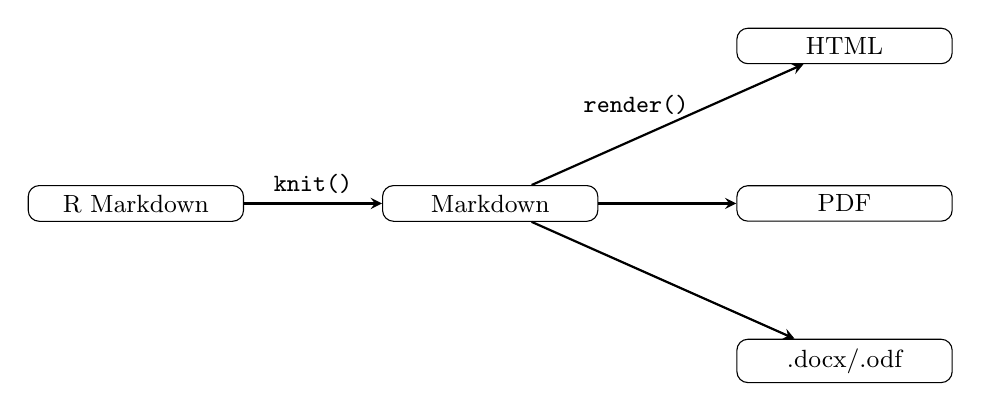
\begin{tikzpicture}
    \node(in)[simple, fill=white, text width=2.5cm]{R Markdown};
    \node(out)[node distance=4.5cm, simple, fill=white, right of=in, text width=2.5cm]{Markdown};
    \node(out1)[node distance=4.5cm, simple, fill=white, right of=out, text width=2.5cm]{PDF};
    \node(out2)[node distance=2cm, simple, fill=white, above of=out1, text width=2.5cm]{HTML};
    \node(out3)[node distance=2cm, simple, fill=white, below of=out1, text width=2.5cm]{.docx/.odf};
    \draw[arrow](in)--node[anchor=south]{\small{\texttt{knit()}}} (out);
    \draw[arrow](out)--(out1);
    \draw[arrow](out)--node[anchor=south, xshift=-4mm]{\small{\texttt{render()}}} (out2);
    \draw[arrow](out)--(out3);
  \end{tikzpicture}
\end{figure}

\section{Introduction}
Phase 1 workflow has provided us with evidence to support the idea of implementing invertibility into reproducible document generation. However the workflow is strictly limited to work on R HTML-based documents, in conjunction with \textbf{knitr}.

R HTML has been the most suitable format to allow us to focus on exploring invertibility, which has been the primary objective of the first phase, but there are other document formats that are potentially more useful. It is of our strong interest to see if the workflow can be more generalised to be applicable for the other useful document formats.

The format we have chosen for the second phase is R Markdown \citep{rmarkdown}, which can be converted to Markdown \citep{markdown} using \textbf{knitr}. There are two main reasons behind our choice of the format; Markdown is rapidly becoming popular and many great tools are available for it.


%-------------------------------------------------------------------------------
\subsubsection*{Popularity}
Markdown is a lightweight markup language that brings simple and readable formatting syntax, unlike the other more sophisticated languages such as TeX and HTML. Because of the simple and readable design, Markdown is gaining popularity amongst many who wish to avoid complexity.

The simplicity, however, does not affect the level of control on the Markdown-based documents as HTML-style markup can be incorporated into the documents to provide HTML exclusive features and controls.


%-------------------------------------------------------------------------------
\subsubsection*{Tools}
Markdown's popularity has influenced many technologies to implement it in their frameworks. Some examples are PageDown \citep{pagedown}, which serves as a parser for Stack Overflow and Stack Exchange websites, and GitHub Flavored Markdown \citep{gfm}, which is used across many features supported in the online project hosting website, GitHub. Many more implementations of Markdown exist across different platforms and languages.

A list of markdown implementations can be found at \url{http://www.w3.org/community/markdown/wiki/MarkdownImplementations}.

Many document conversion tools also exist for Markdown to offer flexible conversion into various document formats. What this flexibility allows us to implement in the workflow is the ability to produce final documents in different formats. For example, a final document can be converted to HTML and PDF, where the former can be published on the Web while the latter can be suitable for printing.

It is possible that our experiment of invertibility on Markdown could bring usable ideas to these implementations and vice versa, which is a sound reason to support our choice.


%-------------------------------------------------------------------------------
\subsubsection*{Demonstration}
Listing \ref{lst:3.1} is the code structure of a simple R Markdown-based source document, \texttt{example2.Rmd}. The highlighted text, lines 13--15, is a R Code Chunk in the R Markdown syntax.

\begin{lstlisting}[caption={\texttt{example2.Rmd}}, escapechar=\|, label={lst:3.1}]
---
title: ""
output:
  html_document:
    toc: false
---

Example
=========================

Summary of the cars data:

|\hl{c}{```\{r\}}|
|\hl{c}{summary(cars)}|
|\hl{c}{```}|
\end{lstlisting}

There is a crucial difference between the two document generation processes of R HTML and R Markdown. R HTML-based documents are knitted \emph{directly} into HTML, whereas R Markdown-based documents are knitted \emph{intermediately} into Markdown, which is then \emph{converted} into the final format. Because there are \emph{two} steps involved in one complete document generation process for R Markdown, the function \texttt{knit()} has to be used twice; firstly on the source R Markdown document and secondly on the knitted Markdown document. The difference is significant but can be overlooked as \textbf{knitr} implements use of the function, \texttt{render()}, from \textbf{rmarkdown} \citep{rmarkdown} package which generates final documents in a single command.

The R code below calls \texttt{render()} to generate the HTML-based final document, \texttt{example2.html}:
\begin{lstlisting}[numbers=none, frame=none]
rmarkdown::render("example2.Rmd", output_format="html_document")
\end{lstlisting}

Listing \ref{lst:3.2} is the code structure of the final document, \texttt{example2.html}. The original R Code Chunk in lines 13--15 of Listing \ref{lst:3.1} is processed to produce the result seen in lines 13--19 of Listing \ref{lst:3.2}. A notable difference is that all elements are now nested in a top-level \texttt{div} element with the class attribute of \texttt{"container-fluid main-container"}.

In general, the HTML document generated from R Markdown has more content, such as \texttt{meta} elements, than the one from R HTML. Note that there are more than one \texttt{meta}, \texttt{script} and \texttt{style} elements inside the \texttt{head} element but these are kept brief in line 4 for simplicity.

\begin{lstlisting}[caption={(tidied) \texttt{example2.html}}, escapechar=\|, label={lst:3.2}]
<!DOCTYPE html>
<html>
<head>
  |\emph{various}| meta, script |\emph{and}| style |\emph{elements.}|
</head>
  <body>
    <style type="text/css"> ... </style>
    <div class="container-fluid main-container">
      <div id="example" class="section level1">
        <h1>Example</h1>
        <p>Summary of the cars data:</p>
        <pre><code>
          ##      speed           dist    
    	  ##  Min.   : 4.0   Min.   :  2  
    	  ##  1st Qu.:12.0   1st Qu.: 26  
    	  ##  Median :15.0   Median : 36  
    	  ##  Mean   :15.4   Mean   : 43  
    	  ##  3rd Qu.:19.0   3rd Qu.: 56  
    	  ##  Max.   :25.0   Max.   :120
    	</code></pre>
      </div>
    </div>
    <script> |\emph{...Bootstrap table styles...}| </script>
    <script> |\emph{... MathJax ...}| </script>    
  </body>
</html>
\end{lstlisting}

Figure \ref{fig:3.1} shows how \texttt{example2.html} looks like in a web browser. Although nearly identical, we can see minor differences between the two final documents, seen in Figures \ref{fig:2.1} and \ref{fig:3.1}, such as different font styles for the headings and spacing used for the R Code Chunk output. These minor differences are due to different \texttt{style} and \texttt{script} elements used in both cases.
\begin{figure}[h!]
% wkhtmltopdf
\fbox{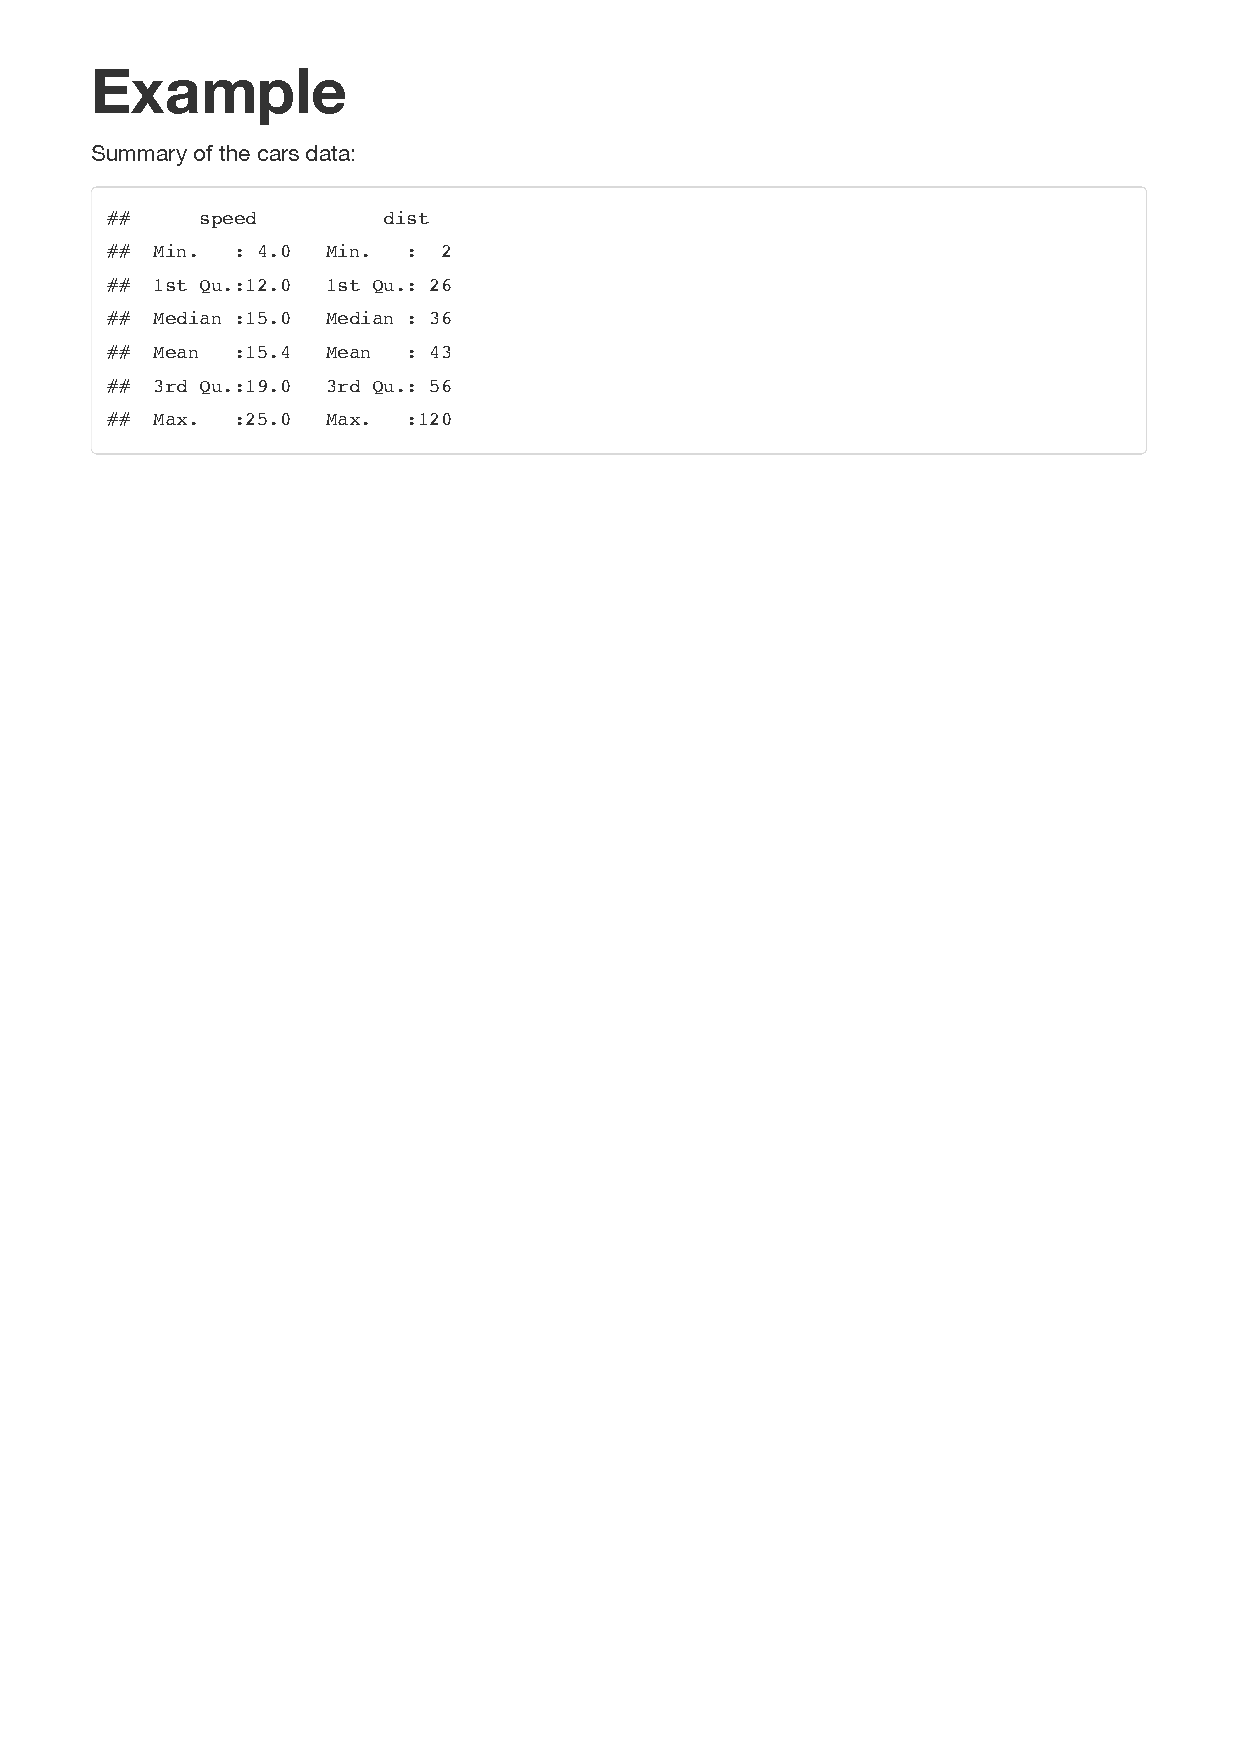
\includegraphics[trim=0cm 22cm 0cm 1cm,clip=true,width=1.1\textwidth,center]{example2}}
\caption{\texttt{example2.html} in a browser}
\label{fig:3.1}
\end{figure}



%------------------------------------------------------------------------------
%--------------------------------- Overview -----------------------------------
%------------------------------------------------------------------------------
\newpage
\section{Overview}
Three additional steps are introduced to phase 2 workflow as a pre-processing stage. Once a source document is pre-processed by the three steps, it becomes reproducible and invertible, and is ready to enter the workflow.

Some of the function names are kept identical to those in phase 1 workflow to minimise confusion and maintain consistency. But it must be noted that there are extra features in these functions that work \emph{exclusively} for R Markdown.

The actual code for the functions can be found at \url{https://github.com/elim1988/honours-project}...

\begin{figure}[h!]
\centering
  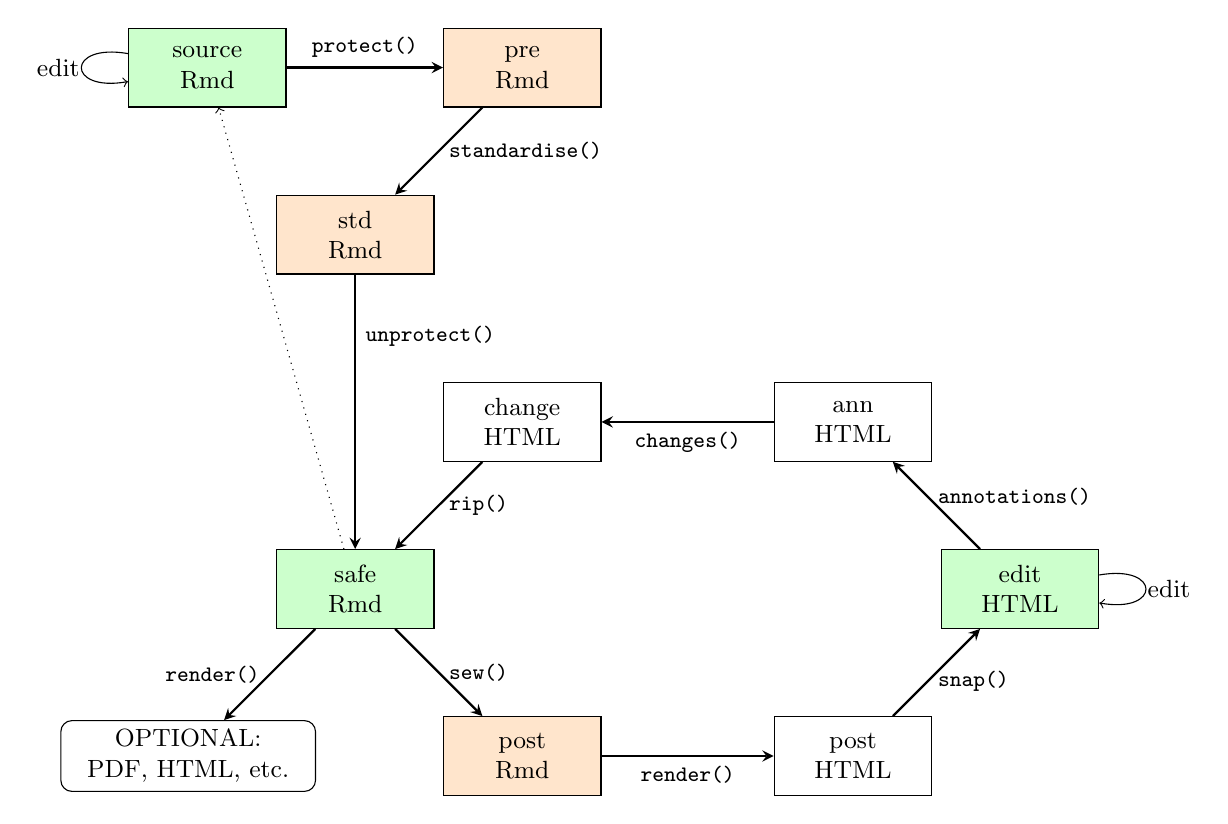
\begin{tikzpicture}
    \node(source)[process, fill=green!20] {source Rmd};
    \node(protect)[node distance=4cm, process, fill=orange!20, right of=source] {pre Rmd};
    \node(standardise)[node distance=3cm, process, fill=orange!20, below left of=protect] {std Rmd};
    \node(start)[node distance=4.5cm, process, fill=green!20, below of=standardise] {safe Rmd};
    \node(sew)[node distance=3cm, process, fill=orange!20, below right of=start] {post Rmd};
    \node(knit)[node distance=4.2cm, process, right of=sew] {post HTML};
    \node(snap)[fill=green!20, node distance=3cm, process, above right of=knit] {edit HTML};
    \node(anno)[node distance=3cm, process, above left of=snap] {ann HTML};
    \node(chgs)[node distance=4.2cm, process, left of=anno] {change HTML};
    %
    \node(output)[simple, node distance=3cm, below left of=start, fill=none] {OPTIONAL: PDF, HTML, etc.};
    \draw[arrow](start) --node[anchor=east] {\footnotesize{\texttt{render()}}} (output);
    %
    \draw[arrow](source) --node[anchor=south] {\footnotesize{\texttt{protect()}}} (protect);
    \draw[arrow](protect) --node[anchor=west] {\footnotesize{\texttt{standardise()}}} (standardise);
    \draw[arrow](standardise) --node[anchor=south west, pos=0.3] {\footnotesize{\texttt{unprotect()}}} (start);
    \draw[arrow](start)--node[anchor=west] {\footnotesize{\texttt{sew()}}} (sew);
    \draw[arrow](sew)--node[anchor=north] {\footnotesize{\texttt{render()}}} (knit);
    \draw[arrow](knit)--node[anchor=west, pos=0.4] {\footnotesize{\texttt{snap()}}} (snap);
    \draw[arrow](snap)--node[anchor=west, pos=0.6] {\footnotesize{\texttt{annotations()}}} (anno);
    \draw[arrow](anno)--node[anchor=north]{\footnotesize{\texttt{changes()}}} (chgs);
    \draw[arrow](chgs)--node[anchor=west] {\footnotesize{\texttt{rip()}}} (start);
    \draw [->] (source) to [loop left, in=190, out=170, distance=8mm] node[anchor=east, xshift=1mm] {\small{edit}} (source);
    \draw [->] (snap) to [loop right, in=350, out=10, distance=8mm] node[anchor=west, xshift=-1mm] {\small{edit}} (snap);
    \draw[->, dotted] (start) to (source);
  \end{tikzpicture}
\caption{Revised reproducible, invertible workflow}
\label{fig:3.2}
\end{figure}


\newpage
%-------------------------------------------------------------------------------
\subsubsection*{Structural differences}
Two final documents of the same format, each generated from \texttt{knit()} and \texttt{render()}, are structurally different. The differences exist for the case of HTML, because R Markdown uses tools such as \textbf{MathJax} \citep{mathjax}, which allows mathematical equations to be specified in LaTeX-style syntax rather than the usual HTML maths syntax, and \textbf{Bootstrap} \citep{bootstrap}, which allows more precise customisation of the layout of the HTML document.

As a result, the \emph{rendered} final document contains more \texttt{script} and \texttt{style} elements than its \emph{knitted} counterpart, as well as different tree structures.

The solution we have chosen to compensate for the differences is to introduce additional steps in the workflow and implement different rules, such as differnt XPath, for the functions of phase 2. These will be discussed in more detail.


%-------------------------------------------------------------------------------
\subsubsection*{Conversion of formats}
\textbf{Pandoc} \citep{pandoc} is the document conversion tool chosen to be implemented in phase 2 workflow due to one main reason; it is fully supported by \textbf{knitr}. In fact, the latest version of \textbf{knitr} comes \emph{with} \textbf{Pandoc}.

It can provide conversion of HTML into Markdown, which is necessary for the final step of the workflow involving the function, \texttt{rip()}.


%-------------------------------------------------------------------------------
\subsubsection*{Invertibility of \textbf{Pandoc}}
\textbf{Pandoc} does not support flawless round trip between two document formats, that is, a source document of one format is not the same as its inverted counterpart of the same format. Figure \ref{fig:3.3} provides a simple diagram to visualise this using Markdown and HTML as the source and intermediary formats, respectively.
\begin{figure}[h!]
\centering
  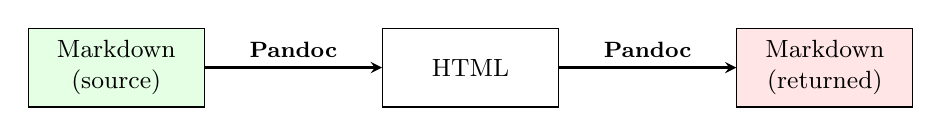
\begin{tikzpicture}[node distance=4.5cm]
    \node(start1)[process, fill=green!10, text width=2cm] {Markdown (source)};
    \node(start2)[process, text width=2cm, right of=start1] {HTML};
    \node(end1)[process, fill=red!10, right of=start2, text width=2cm] {Markdown (returned)};
    \draw[arrow](start1)--node[anchor=south] {\footnotesize{\textbf{Pandoc}}} (start2);
    \draw[arrow](start2)--node[anchor=south] {\footnotesize{\textbf{Pandoc}}} (end1);
  \end{tikzpicture}
\caption{The two Markdown documents are structurally different.}
\label{fig:3.3}
\end{figure}

The cause of this occurrence is due to the existence of an internal structure in \textbf{Pandoc} that determines the structure of its output documents. This means that whether the source document obeys the internal structure or not, \textbf{Pandoc} will always produce a final document that follows the internal structure, i.e., it \emph{standardises}. This is best understood with a simple diagram:
\begin{figure}[h!]
\centering
  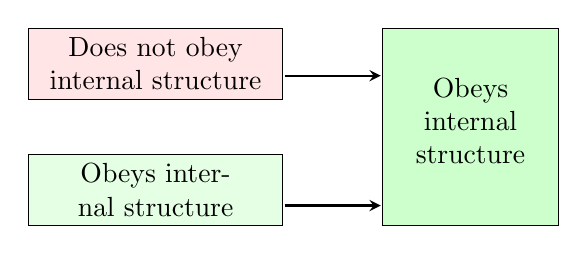
\begin{tikzpicture}
  	\node[draw, fill=green!20, text width=2cm, text height=3cm, text centered, text height=5ex, text depth=10ex] (end) at (4,0) {Obeys internal structure};
  	\node[draw, fill=red!10, left=4cm of end.north, anchor=north, text width=3cm, text centered] (start1) {Does not obey internal structure};
  	\node[draw, fill=green!10, left=4cm of end.south, anchor=south, text width=3cm, text centered] (start2) {Obeys internal structure};
  	\draw[arrow](1.64,0.65)--(2.86,0.65);
  	\draw[arrow](1.64,-1)--(2.86,-1);
  \end{tikzpicture}
\caption{Standardisation of \textbf{Pandoc}}
\end{figure}

We have decided to use the internal structure as a means of \emph{standardising} the source document so that any subsequent conversion by \textbf{Pandoc} does not interfere with its structure. The structural integrity of standardised documents will be consistent throughout the workflow.

The standardisation step is carried out by the function, \texttt{standardise()} with the use of \textbf{Pandoc}.


%-------------------------------------------------------------------------------
\subsubsection*{Editing source documents}
Because of the requirement for standardisation, an inverted document must be standardised each time it runs through the workflow. This is indicated by the dotted arrow in Figure \ref{fig:3.2}.


%-------------------------------------------------------------------------------
\subsubsection*{Loss of information 2}
R Markdown has syntax for specifying (YAML) metadata, such as author, title and date information. An example of a metadata section is as below:
\begin{lstlisting}[numbers=none, frame=none]
---
title: "Example"
output:
  html_document:
    toc: true
    theme: united
---
\end{lstlisting}

Metadata sections are \emph{exclusive} to R Markdown. As a result, \textbf{Pandoc} discards them in its output documents. This means that the metadata information cannot be carried over to subsequent steps after the standardisation step. \textbf{Pandoc} also interferes with R Code Chunks in R Markdown, because R Code Chunks are not known to \textbf{Pandoc}.  The solution we have chosen is to implement a pre-processing step to protect the metadata sections and R Code Chunks.

The usual delimiters, \texttt{---}, for metadata are changed to \texttt{<!--rmd\_metadata} and \texttt{rmd\_metadata--> rmd-rmLines}. The protected version of the previous metadata example is as below:
\begin{lstlisting}[numbers=none, frame=none]
<!--rmd_metadata
title: "Example"
output:
  html_document:
    toc: true
    theme: united
rmd_metadata--> rmd-rmLines
\end{lstlisting}

R Code Chunks are protected by \texttt{<!--begin.keepcode} and \texttt{end.keepcode--> rmd-rmLines} delimiters.

The function, \texttt{protect()}, carries out the protection of metadata and R Code Chunks.


%-------------------------------------------------------------------------------
\subsubsection*{Optional pathway}
Once the final version of a document is achieved, there is an optional path using the function, \texttt{render()}, to produce the final document in different formats.

The optional path is indicated by the ``OPTIONAL" node in Figure \ref{fig:3.2}.



%-------------------------------------------------------------------------------
%------------------------------ Functions detail -------------------------------
%-------------------------------------------------------------------------------
\newpage
\section{Functions detail}
\subsubsection*{\texttt{protect()}}
The function \emph{protects} metadata sections and R Code Chunks in the source document.

Metadata sections are delimited by \texttt{<!--rmd\_metadata} and \texttt{rmd\_metadata--> rmd-rmLines}.

R Code Chunks are delimited by \texttt{<!--begin.keepcode} and \texttt{end.keepcode--> rmd-rmLines}.

The use of \texttt{rmd-rmLines} is to correct for \textbf{Pandoc}'s tendency of removing empty lines after the protected lines.

The default suffix of the output file is \texttt{.pre.Rmd}, converted from the source suffix, \texttt{.Rmd}.

Listing \ref{lst:3.3} is the code structure of the protected source document, \texttt{example2.pre.Rmd}.
\begin{lstlisting}[caption={\texttt{example2.pre.Rmd}}, label={lst:3.3}, escapechar=\|]
|\hl{c}{<!--rmd\_metadata}|
title: ""
output:
  html_document:
    toc: false
|\hl{c}{rmd\_metadata--> rmd-rmLines}|

Example
=========================

Summary of the cars data:

|\hl{c}{<!--begin.keepcode}|`|`|`|{r, echo=FALSE|}
summary(cars)
|`|`|`||\hl{c}{end.keepcode--> rmd-rmLines}|
\end{lstlisting}


%-------------------------------------------------------------------------------
\subsubsection*{\texttt{standardise()}}
The function calls \textbf{Pandoc} to \emph{standardise} the protected source document. In this function, \texttt{system()} is used to invoke the command line necessary for calling \textbf{Pandoc}.

The default suffix of the output file is \texttt{.std.Rmd}, converted from the input suffix, \texttt{.pre.Rmd}.

Listing \ref{lst:3.4} is the code structure of the standardised source document, \texttt{example2.std.Rmd}. A couple of things to note is that the equal signs in line 10, which correspond to R Markdown's syntax for specifying a heading, are reduced in length, and the delimiters, \texttt{rmd-rmLines}, are broken into the next lines in lines 7 and 17. These are some of the examples of \textbf{Pandoc}'s internal structure.
\begin{lstlisting}[caption={\texttt{example2.std.Rmd}}, escapechar=\|, label={lst:3.4}]
<!--rmd_metadata
title: ""
output:
  html_document:
    toc: false
rmd_metadata-->
|\hl{c}{rmd-rmLines}|

Example
|\hl{c}{=======}|

Summary of the cars data:

<!--begin.keepcode```{r, echo=FALSE}
summary(cars)
```end.keepcode-->
|\hl{c}{rmd-rmLines}|
\end{lstlisting}


%-------------------------------------------------------------------------------
\subsubsection*{\texttt{unprotect()}}
The function removes the protection added by \texttt{protect()}.

The special delimiters used to protect metadata and R Code Chunks are reverted back to their normal R Markdown syntax.

The pushed down lines for \texttt{rmd-rmLines} delimiters are simply removed.

The default suffix of the output file is \texttt{.safe.Rmd}, converted from the input suffix, \texttt{.std.Rmd}.

Listing \ref{lst:3.5} is the code structure of the standardised invertible document, \texttt{example2.safe.Rmd}.
\begin{lstlisting}[caption={\texttt{example2.safe.Rmd}}, escapechar=\|, label={lst:3.5}]
---
title: ""
output:
  html_document:
    toc: false
---

Example
=======

Summary of the cars data:

```{r, echo=FALSE}
summary(cars)
```
\end{lstlisting}

We can use the \texttt{diff} command below to compare the source document, \texttt{example2.Rmd}, and the invertible source document, \texttt{example2.safe.Rmd}:
\begin{lstlisting}[numbers=none, frame=none]
$ diff example2.Rmd example2.safe.Rmd
\end{lstlisting}

Listing \ref{lst:3.6} is the output form the previous \texttt{diff} command. The only difference between the two source documents is line 9, where the number of equal signs is reduced by the internal structure of \textbf{Pandoc}.
\begin{lstlisting}[caption={Output from \texttt{diff}}, label={lst:3.6}]
9c9
< =========================
---
> =======
\end{lstlisting}


%-------------------------------------------------------------------------------
\subsubsection*{\texttt{sew()}}
The function carries out a similar pre-processing step as the phase 1 version with one addition; it copies metadata sections (as well as R Code Chunks) and append the copies after their originals.

The default suffix of the output file is \texttt{.post.Rmd}, converted from the input suffix, \texttt{.safe.Rmd}.

%-------------------------------------------------------------------------------
\subsubsection*{\texttt{render()}}
The function is directly from the R package, \texttt{rmarkdown}. This function is what \textbf{knitr} uses to convert R Markdown-based source documents into final documents. In fact, the latest version of \textbf{knitr} is included with \textbf{rmarkdown}.

The default suffix of the output file is \texttt{.post.html}, converted from the input suffix, \texttt{post.Rmd}.

%-------------------------------------------------------------------------------
\subsubsection*{\texttt{snap()}}
The function carries out conceptually the same tasks as the phase 1 version; add pieces of HTML and JavaScript code to the final document, and add HTML attributes to editable nodes. But different rules are used for phase 2 \texttt{snap()}.

The JavaScript code, that loads \textbf{jQuery}, \textbf{CKEditor} and \textbf{Annotator}, is appended at the end of other \texttt{script} elements that are added by \texttt{render()} to avoid interference from them.

Because of the differences in the tree structure, the location of editable elements is different. They are nested in a top-level \texttt{div} element with the \texttt{class} attribute, \texttt{"container-fluid main-container"}. If there is at least one heading, all elements under the heading are further nested inside another \texttt{div} element with \texttt{id} attribute of the heading name. Thus different XPath is used to locate the editable elements and add \texttt{contenteditable} and \texttt{id} attributes accordingly.

Once the editable document is successfully obtained, it can be uploaded on the test server for editing, similarly to the phase 1 procedure.

The default suffix of the output file is \texttt{.edit.html}, converted from the input suffix, \texttt{.post.html}.

Listing \ref{lst:3.7} is the code structure of the editable final document, \texttt{example2.edit.html}.
\begin{lstlisting}[caption={(tidied) \texttt{example2.edit.html}}, escapechar=\|, label={lst:3.7}]
<!DOCTYPE html>
<html>
<head>
  |\emph{various}| meta, script |\emph{and}| style |\emph{elements.}|
</head>
  <body>
    <style type="text/css"> ... </style>
    <div class="container-fluid main-container">
      <div id="example" class="section level1">
        <!--rmd_metadata
        title: ""
        output:
          html_document:
            toc: false
        rmd_metadata-->
        <h1 contenteditable="true" id="Editor-1">Example</h1>
        <p contenteditable="true" id="Editor-2">Summary of the cars data:</p>
        <pre><code>
          ##      speed           dist    
    	  ##  Min.   : 4.0   Min.   :  2  
    	  ##  1st Qu.:12.0   1st Qu.: 26  
    	  ##  Median :15.0   Median : 36  
    	  ##  Mean   :15.4   Mean   : 43  
    	  ##  3rd Qu.:19.0   3rd Qu.: 56  
    	  ##  Max.   :25.0   Max.   :120
    	  <!--begin.keepcode```{r, echo=FALSE}
    	  summary(cars)
    	  ```end.keepcode-->
    	</code></pre>
      </div>
    </div>
    <script> |\emph{...Bootstrap table styles...}| </script>
    <script> |\emph{... MathJax ...}| </script>    
  </body>
</html>
\end{lstlisting}


%-------------------------------------------------------------------------------
\subsubsection*{\texttt{annotations()}}
Only one aspect of the function differs from its phase 1 counterpart due to the differences in the tree structure.

All R-created contents are included in \texttt{code} elements, nested in \texttt{pre} elements, instead of \texttt{div} elements with \texttt{class="chunk"} attribute for phase 1. Hence different XPath is used to locate these sections of R-created contents and insert annotations accordingly.

The default suffix of the output file is \texttt{.anns.html}, converted from the input suffix, \texttt{.edit.html}.

Listing \ref{lst:3.8} is the code structure of the annotated final document, \texttt{example2.anns.html}, using the same annotation as the previous example.
\begin{lstlisting}[caption={(tidied) \texttt{example2.anns.html}}, escapechar=\|, label={lst:3.8}]
<!DOCTYPE html>
<html>
<head>
  |\emph{various}| meta, script |\emph{and}| style |\emph{elements.}|
</head>
  <body>
    <p id="savebutton" style="background-color:grey; text-align:center">
      <button onclick="savechanges()">save</button>
    </p>
    <style type="text/css"> ... </style>
    <div class="container-fluid main-container">
      <div id="example" class="section level1">
        <!--rmd_metadata
        title: ""
        output:
          html_document:
            toc: false
        rmd_metadata-->
        <h1 contenteditable="true" id="Editor-1">Example</h1>
        <p contenteditable="true" id="Editor-2">Summary of the cars data:</p>
            |\hl{c}{<p class="annotation" style = "background-color:coral">}|
            |\hl{c}{<em>Annotation: The text "speed" was annotated with the}|
            |\hl{c}{message "need units"</em></p>}|
        <pre><code>
          ##      speed           dist    
    	  ##  Min.   : 4.0   Min.   :  2  
    	  ##  1st Qu.:12.0   1st Qu.: 26  
    	  ##  Median :15.0   Median : 36  
    	  ##  Mean   :15.4   Mean   : 43  
    	  ##  3rd Qu.:19.0   3rd Qu.: 56  
    	  ##  Max.   :25.0   Max.   :120
    	  <!--begin.keepcode```{r, echo=FALSE}
    	  summary(cars)
    	  ```end.keepcode-->
    	</code></pre>
      </div>
    </div>
    <script> |\emph{...Bootstrap table styles...}| </script>
    <script> |\emph{... MathJax ...}| </script>    
  </body>
</html>
\end{lstlisting}


%-------------------------------------------------------------------------------
\subsubsection*{\texttt{changes()}}
The function is identical to its phase 1 counterpart, except that it uses different XPath to correct for the different tree structure.

The default suffix of the output file is \texttt{.save.html}, converted from the input suffix, \texttt{.anns.html}.

Listing \ref{lst:3.9} is the code structure of the final document merged with the change, same as the previous example.
\begin{lstlisting}[caption={(tidied) \texttt{example2.save.html}}, escapechar=\|, label={lst:3.9}]
<!DOCTYPE html>
<html>
<head>
  |\emph{various}| meta, script |\emph{and}| style |\emph{elements.}|
</head>
  <body>
    <p id="savebutton" style="background-color:grey; text-align:center">
      <button onclick="savechanges()">save</button>
    </p>
    <style type="text/css"> ... </style>
    <div class="container-fluid main-container">
      <div id="example" class="section level1">
        <!--rmd_metadata
        title: ""
        output:
          html_document:
            toc: false
        rmd_metadata-->
        <h1 contenteditable="true" id="Editor-1">Example</h1>
        <p contenteditable="true" id="Editor-2">
        |\hl{c}{<code>summary(cars):</code>}|
        </p>
            <p class="annotation" style = "background-color:coral">
            <em>Annotation: The text "speed" was annotated with the
            message "need units"</em></p>
        <pre><code>
          ##      speed           dist    
    	  ##  Min.   : 4.0   Min.   :  2  
    	  ##  1st Qu.:12.0   1st Qu.: 26  
    	  ##  Median :15.0   Median : 36  
    	  ##  Mean   :15.4   Mean   : 43  
    	  ##  3rd Qu.:19.0   3rd Qu.: 56  
    	  ##  Max.   :25.0   Max.   :120
    	  <!--begin.keepcode```{r, echo=FALSE}
    	  summary(cars)
    	  ```end.keepcode-->
    	</code></pre>
      </div>
    </div>
    <script> |\emph{...Bootstrap table styles...}| </script>
    <script> |\emph{... MathJax ...}| </script>    
  </body>
</html>
\end{lstlisting}

Figure \ref{fig:3.5} shows how the \emph{annotated} and \emph{changed} final document, \texttt{exampe2.save.html} looks like in a web browser.
\begin{figure}[h]
\includegraphics[trim=0cm 19.6cm 0cm 1.8cm,clip=true,width=1\textwidth,center]{example2-save}
\caption{\texttt{example2.save.html}}
\label{fig:3.5}
\end{figure}


%-------------------------------------------------------------------------------
\subsubsection*{\texttt{rip()}}
The function carries out \emph{two} additional steps; one of which uses \textbf{Pandoc} to remove the unwanted contents and the other to tidy up before inverting source documents.

The first stage of the function is to remove \emph{some} of the unwanted contents, such as the two attributes added to editable elements.

The second stage uses \textbf{Pandoc} to remove the rest of the unwanted contents, in a similar manner to the standardisation step of the workflow. This method has been implemented in \texttt{rip()} because \textbf{Pandoc} removes the unwanted contents, such as various \texttt{script} and \texttt{style} elements relatively easily and much more robustly than the text processing approach used in phase 1.

The third stage involves adjustments necessary to \emph{tidy} up the document to complete the inversion process.

The default suffix of the output file is \texttt{.return.Rmd}, converted from the input suffix, \texttt{.save.html}.

Listing \ref{lst:3.10} is the code structure of the inverted document, \texttt{example2.return.Rmd}. Note that the back-ticks seen in line 11 are the syntax for specifying code style, and the asterisks seen in line 13 are the syntax for italicising.
\begin{lstlisting}[caption={\texttt{example2.return.html}}, escapechar=\|, label={lst:3.10}]
---
title: ""
output:
  html_document:
    toc: false
---

Example
=======

`summary(cars):`

*Annotation: The text "speed" was annotated with the message "need units"*

```{r, echo=FALSE}
summary(cars)
```
\end{lstlisting}

And finally, the \texttt{diff} command below can be used to compare the source and the inverted documents, \texttt{example2.Rmd} and \texttt{example2.return.Rmd}.
\begin{lstlisting}[frame=none, numbers=none]
$ diff example2.Rmd example2.return.Rmd
\end{lstlisting}

Listing \ref{lst:3.11} is the output from the previous \texttt{diff} command that suggests the only differences are the lines corresponding to the merged change and annnotation.
\begin{lstlisting}[caption={Output from \texttt{diff}}, label={lst:3.11}]
11c11,13
< Summary of the cars data:
---
> `summary(cars):`
> 
> *Annotation: The text "speed" was annotated with the message "need units"*
\end{lstlisting}



%------------------------------------------------------------------------------
%-------------------------------- Discussion ----------------------------------
%------------------------------------------------------------------------------
\chapter{Discussion}
We have described a couple of workflows, each of which is specific to work with one  particular type of source document, that allows a consultant to write a report as invertible and reproducible, a client to edit and annotate directly on the report and the corrected report to be inverted back to the source format with the change and annotation merged.

Phase 1 workflow has brought some plausible ideas that an invertible workflow can be implemented in reproducible document generation. By no means is the workflow production-quality nor can it be readily substituted for another pre-exisiting well established workflow, but its strength lies in demonstrating the concept of invertibility and providing a departing point for further exploration.

Phase 2 workflow has provided some evidence towards the possibility of generalising the invertible workflow. Again it is not of production-quality, but it has shown that further generalisation is achievable with greater effort.

The rest of this chapter includes limitations associated with the workflows, comparisons with other workflows and tools, and suggestions for generalising them.

%-------------------------------------------------------------------------------
%--------------------------------- Limitations ---------------------------------
%-------------------------------------------------------------------------------
\section*{Limitations}
The main limitation comes from the fact that the functions, involved in the workflows, are tightly \emph{coupled} with the tools implemented in the workflows, i.e., their functionality depends on the use of this particular combination of the tools.

A direct consequence from the high coupling is that the functions are not very general; they are \emph{specific} to work only with \textbf{knitr}, \textbf{CKEditor}, \textbf{Annotator} and \textbf{Pandoc}. An attempt at replacing these tools with different tools will not be successful unless appropriate adjustments are made for the functions.

Another consequence is that the functions are fragile; they are defenceless against changes in the underlying tools. Most of the functions work on the assumptions, or expectations, that these tools behave in certain \emph{patterns}, e.g., \textbf{Annotator} only works on particular \texttt{div} elements that should be annotatable based on the assumption that \texttt{knit()} consistently puts all R-created contents in these elements. It can be problematic if changes are introduced in the tools, possibly with an update, to alter these assumptions.

Other limitations include difficulties with providing editable environment for images, tables and equations and dealing with these elements in general. These particular limitations could be associated with our choice of HTML as the format, as opposed to TeX-based Rnw format that may easily avoid these limitations. However HTML offers benefits such as \emph{interactivity} which is not as easily accessible using Rnw.

Phase 2 specific limitations are that the functions are not based on all of the R Markdown's syntax, such as HTML markup within R Markdown, and that only some of the internal structure of \textbf{Pandoc} has been considered.

All of these limitations could be potentially avoided by generalising the workflows so that alternative more feature-rich tools can be implemented. A possible solution to improve the fragile defence of the functions is to implement an automated syncing process in them so they can always work on most up-to-date patterns.


%-------------------------------------------------------------------------------
%-------------------------- Other workflows and tools --------------------------
%-------------------------------------------------------------------------------
\section*{Other workflows and tools}
Phase 1 and 2 workflows are designed to implement the idea of invertibility; their design focus is predominantly in inverting final documents.

Beyond this restrictive design, there are many reproducible document workflows, which may not be invertible but are worth introducing for comparisons and to generate ideas for future direction of the project.

Also there are many alternative tools to \textbf{knitr} for consideration.


\subsubsection*{Shared document workflow}
\begin{figure}[h!]
\centering
  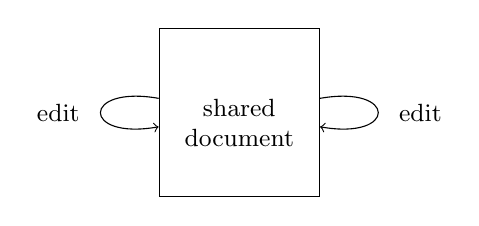
\begin{tikzpicture}
    \node(doc)[process, text width=1.8cm, text height=1cm, text depth=6ex] {shared document};
    \draw [->] (doc) to [loop left, in=190, out=170, distance=1cm] (doc) node[anchor=north, left of=doc, xshift=-1.3cm] {\small{edit}};
    \draw [->] (doc) to [loop right, in=350, out=10, distance=1cm] (doc) node[anchor=west, right of=doc, xshift=1.3cm] {\small{edit}};
  \end{tikzpicture}
\end{figure}

Shared document workflows involve editing on a single document, i.e., the source and final documents are the same. Once a final document is generated, it can be edited indefinitely. A notable package in R to implement a shared document workflow is \textbf{SWord} (REF), where final documents are generated as Word documents. Another tool is \textbf{RExcel} (REF) that provides a shared document workflow in Excel.

This type of workflow is best suited for collaborative work that requires no version control, e.g., collaborative research amongst professionals where changes do not require thorough examination and investigation before merging.

The fundamental problem that we are trying to solve in this project, that is the aforementioned client-consultant situation, is completely avoided in a shared document workflow; clients and consultants work on the same document. The whole purpose of being a client or a consultant is defeated.

However the shared document workflow is usually more efficient as it does not require inversion steps, and collaboration makes them more productive. These advantages are something to consider for the invertible workflows to implement in future.

Beyond the R environment, \textbf{IPython notebooks} \citep{ipython} and \textbf{R Extensions for MediaWiki} \citep{rextension} are two notable tools that implement shared document workflows.


\subsubsection*{Workflows based on other formats}
There are countless packages and tools to provide reproducible document workflows based on different document formats.

One example is an R package, \textbf{odfWeave} \citep{odfweave}, which provides an Open Office-based reproducible workflow.

More R packages to provide alternative workflows can be found at \url{http://cran.r-project.org/web/views/ReproducibleResearch.html}.


\subsubsection*{Predecessors of knitr}
The dynamic report generation tool, \textbf{knitr}, is essentially the summation of various pre-existing packages along with improvements and add-ons. These pre-dating packages include \textbf{Sweave} \citep{sweave} and \textbf{R2HTML} \citep{r2html}, both of which offer reproducible document generation based on HTML as final documents.

Depending on the structural complexity of the final documents generated using these tools, it seems highly plausible that the invertible workflows can work with either or both of these tools with minor adjustments.


\subsubsection*{Alternatives of knitr}
R packages such as \textbf{hwriterPlus} \citep{hwriterplus} and \textbf{ReporteRs} \citep{reporters} also offer reproducible report generation in HTML.

\textbf{ReporteRs} requires particular attention as it can add R plots as editable vector graphics in the final documents to allow viewers to directly modify the plots.

The difficulties associated with images and plots could be overcome by implementing such a package in an invertible workflow.





%-------------------------------------------------------------------------------
%-------------------------------- Generalisation -------------------------------
%-------------------------------------------------------------------------------
\section*{Generalisation}
Generalising the invertible workflows can help relieve their restrictions to work only with HTML documents, which can potentially improve their usability.

This section considers possibility of generalising the invertible workflows.


\subsubsection*{Beyond CKEditor and Annotator}
It may be obvious that many other JavaScript libraries are better and more robust than \textbf{CKEditor} and \textbf{Annotator}. But there are useful aspects of these libraries which might not be present in others.

A useful aspect of \textbf{CKEditor} is the ability to provide an editable GUI for \emph{each} section, which might be a difficult feature to replicate in other tools.

\textbf{Annotator} has been useful as it provides more detailed information than needed, which is more advantageous than lacking in information.

It may be worthwhile to consider whehter JavaScript libraries to replace \textbf{CKEditor} and \textbf{Annotator} can offer similar features beforehand.


\subsubsection*{Beyond HTML}
Although phase 2 workflow has suggested that Markdown-based workflows can be invertible, there are still many other document formats to consider.

One of the most desirable format is TeX-based Rnw. However it seems highly unlikely that Rnw-based invertible workflow is possible due to complications in inverting PDF files into Rnw-based source code.


\subsubsection*{Beyond client-consultant situation}
The invertible workflows described in this report are motivated by the previously mentioned client-consultant scenario.

An invertible workflow is suitable for this particular situation because the levels of programmatic and technical skills vary widely between clients and consultants.

They can be extended to bring relevance in other contexts such as scientific reproducibility, where similar situations can often arise.


\subsubsection*{Extending R}
Having to annotate on the sections of R-created contents is a restriction that is only a temporary solution to deal with the issues of losing and gaining of information.

If R itself can be extended to be hosted on the test server, in a similar manner to \textbf{R Extensions for MediaWiki}, R Code Chunks can be directly edited and run to observe different output.

Extremely robust version control system must then be implemented as it can be difficult to keep track of which code is changed or left alone.


%------------------------------------------------------------------------------
\chapter{Conclusion}
Our ultimate goal remains to be in further generalising the round trip to suit a broader spectrum of document types.

Phase 1 workflow has contributed evidence that invertible reproducible document generation is possible.

Phase 2 workflow has suggested that the invertible reproducible document generation can be general to a certain degree.

Although these workflows are not to be readily integrated into commercial world, the ideas described in this report are hopefully useful for people who are passionate about document generation and value reproducible research.


%------------------------------------------------------------------------------
\section*{Contributions}
The project supervisors contributed with various ideas and guidance.

The functions, \texttt{sew()}, \texttt{snap()}, \texttt{annotate()}, \texttt{changes()} and \texttt{rip()}, are developed by the author.

Paul Murrell wrote the JavaScript code for loading \textbf{CKEditor} and \textbf{Annotator}, and set up the test server.

Finlay Thompson provided the original problem statement.


\section*{Further reading}




\bibliography{final_report}{}
\bibliographystyle{plainnat}

\end{document}
